\documentclass{article}
\usepackage[table]{xcolor}
\usepackage[T1]{fontenc}
\usepackage{tgschola}
\usepackage[a4paper, total={6in, 8in}, margin=2cm]{geometry}
\usepackage{lipsum}
\usepackage{fancyhdr}
\usepackage{lastpage}
\setlength{\headheight}{48.2pt}
\usepackage{boxedminipage}
\usepackage{graphicx}
\usepackage{tikz}
\usetikzlibrary{shapes.geometric}
\usepackage{wrapfig}
\usepackage{float}
\usepackage{subfig}
\usepackage{circuitikz}
\usetikzlibrary{arrows}
\usepackage[T1]{fontenc}
\usepackage{tgbonum}
\usepackage[most]{tcolorbox}
\usepackage{textgreek}
\usepackage{graphicx}
\graphicspath{ {./} }
\usepackage[T1]{fontenc}
\usepackage{multicol}
\usepackage{siunitx}
\sisetup{output-decimal-marker = {,}} %para que use coma en vez de punto
\usepackage[usestackEOL]{stackengine}
\graphicspath{ {./imagenes/} }
\pagestyle{fancy}
\usepackage{enumitem}
\usepackage[most]{tcolorbox}
\usepackage[option ]{askmaps}
\usepackage{circuitikz}
\usepackage{float}
\usepackage{adjustbox}
\usepackage{amsmath}
\usepackage{array}
\usepackage{multirow}
\usepackage{geometry}
\usepackage{booktabs}
\usepackage{tikz-timing}
\usepackage{url}

\definecolor{headergray}{RGB}{220,220,220}
\usepackage{geometry}
\usepackage{changepage}
\usepackage{listings}
\lstset{
	basicstyle=\small\ttfamily,
	columns=flexible,
	breaklines=true
}
\usepackage{skull}
\usepackage{makecell}
\usetikzlibrary {arrows.meta,automata,positioning}


%%Modificar los siguientes valores segun la materia/tp
\newcommand{\Titulo}{Trabajo Práctico 5}
\newcommand{\Subtitulo}{Máquinas de estado finito }
%\newcommand{\SubtituloDos}{y Aritmética binaria}
\newcommand{\Version}{Versión 261C.01}
\newcommand{\Carrera}{INGENIERÍA EN INFORMÁTICA}
\newcommand{\Asignatura}{3631 - Fundamentos de sistemas embebidos}
\newcommand{\Tema}{FSM Hardware y Software (Micropython)}
\newcommand{\Unidad}{5.0 $\sim$ 5.1}
\newcommand{\Objetivo}{Diseñar máquinas de estado integrando los conocimientos de lógica combinacional y secuencial}
\newcommand{\TiempoResolucion}{2 semanas}
\newcommand{\Metodologia}{Ejercicios verificados en simuladores}
\newcommand{\Entrega}{No obligatoria}


\fancyhead[L]{\framebox(128,64){\includegraphics[scale=0.18]{diit}}}
\fancyhead[C]{\framebox(224,64){\Longstack{\textbf{\Titulo}\\\textbf{\Subtitulo}\\Pág. \thepage\ de \pageref{LastPage}}}}
\fancyhead[R]{\framebox(128,64){\includegraphics[scale=0.055]{logo}}}
\renewcommand{\headrulewidth}{0.0pt}
\renewcommand{\footrulewidth}{0pt}



\begin{document}
	
	\centering\LARGE{\textbf{\Version}}
	\large
	\\
	\begin{center}
		\begin{tabular}{|p{16cm}|} % 'l' for left-aligned, 'p' for paragraph with specified width
			
			\hline
			\rule{0pt}{15pt}
			\textbf{Carrera: \Carrera} \\
			\hline
			\rule{0pt}{15pt}
			\textbf{Asignatura:}  \Asignatura \\
			\hline
			\rule{0pt}{15pt}
			\textbf{Tema:}  \Tema \\
			\hline
			\rule{0pt}{15pt}
			\textbf{Unidad:}  \Unidad \\
			\hline
			\rule{0pt}{15pt}
			\textbf{Objetivo:} \Objetivo \\
			\hline
			\rule{0pt}{15pt}
			\textbf{Competencias a desarrollar:} 
			\begin{itemize}
				\item Concepción, diseño y desarrollo de proyectos de ingeniería en informática.
				\item Gestión, planificación, ejecución y control de proyectos de ingeniería en informática.
				\item Utilización de técnicas y herramientas de aplicación en la ingeniería en informática.
				\item Generación de desarrollos tecnológicos y/o innovaciones tecnológicas.
				\item Desarrollo de una actitud profesional emprendedora.
				\item Aprendizaje continuo
				\item Actuación profesional ética y responsable.
				\item Comunicación efectiva.
				\item Desempeño en equipos de trabajo.
				\item Identificación, formulación y resolución de problemas de ingeniería en informática
			\end{itemize} \\
			\hline
			\rule{0pt}{15pt}
			\textbf{Descripción de la actividad:} 
			\begin{enumerate}
				\item  Tiempo estimado de resolución: \TiempoResolucion
				\item Metodología: \Metodologia
				\item Forma de entrega: \Entrega
				\item Metodología de corrección y feedback al alumno: Presencial y por Miel.
			\end{enumerate} \\
			\hline
		\end{tabular}
	\end{center}
	
	\clearpage
	
	%% Hacer que las tablas tengan un poco de padding
	\def\arraystretch{1.2}
	
	\section*{F- Máquinas de Estado Finito (FSM) Hardware}	
	
	\begin{enumerate}[label=\textbf{F.\arabic*}]
		\item Utilizando un contador binario sincrónico ascendente de 3 bits (simil hoja 3 de la teoría)
		implemente un \textbf{secuenciador} que genere el siguiente código: 0000 → 0001 → 0011 → 0111
		→ 1111 → 1110 → 1100 → 1000. Grafique en logisim utilizando el osciloscopio digital. \\
		\begin{tikzpicture}[x=1pt,y=-1pt,line cap=rect]
			\def\logisimfontA#1{\fontfamily{cmr}{#1}} % Replaced by logisim, original font was "SansSerif"
			\def\logisimfontB#1{\fontfamily{Dialog}{#1}}
			\definecolor{custcol_b2_b2_b2}{RGB}{178, 178, 178}
			\definecolor{custcol_0_91_91}{RGB}{0, 145, 145}
			\definecolor{custcol_0_64_0}{RGB}{0, 100, 0}
			\definecolor{custcol_fa_fa_fa}{RGB}{250, 250, 250}
			\definecolor{custcol_0_0_0}{RGB}{0, 0, 0}
			\definecolor{custcol_0_d0_d0}{RGB}{0, 208, 208}
			\definecolor{custcol_40_40_40}{RGB}{64, 64, 64}
			\definecolor{custcol_ff_ff_ff}{RGB}{255, 255, 255}
			\definecolor{custcol_0_46_46}{RGB}{0, 70, 70}
			\definecolor{custcol_80_80_80}{RGB}{128, 128, 128}
			\definecolor{custcol_0_65_65}{RGB}{0, 101, 101}
			\definecolor{custcol_28_28_ff}{RGB}{40, 40, 255}
			\draw [line width=3.0pt, custcol_0_64_0 ]  (85.0,346.0) -- (85.0,356.0) ;
			\draw [line width=3.0pt, custcol_0_64_0 ]  (55.0,16.0) -- (85.0,16.0) ;
			\draw [line width=4.0pt, custcol_0_0_0 ]  (305.0,106.0) -- (315.0,106.0) -- (335.0,106.0) ;
			\draw [line width=3.0pt, custcol_0_64_0 ]  (45.0,206.0) -- (55.0,206.0) ;
			\draw [line width=4.0pt, custcol_0_0_0 ]  (315.0,106.0) -- (315.0,156.0) -- (5.0,156.0) -- (5.0,336.0) -- (25.0,336.0) ;
			\draw [line width=4.0pt, custcol_0_0_0 ]  (305.0,16.0) -- (315.0,16.0) -- (315.0,76.0) -- (75.0,76.0) -- (75.0,106.0) -- (85.0,106.0) ;
			\fill [line width=4.0pt, custcol_0_0_0]  (315.0,106.0) ellipse (6.0 and 6.0 );
			\fill [line width=1.0pt, custcol_0_0_0 ]  (85.0,15.0) rectangle (95.0,18.0) ;
			\logisimfontB{\fontsize{12pt}{12pt}\selectfont\node[inner sep=0, outer sep=0, custcol_40_40_40, anchor=base west] at  (100.0,20.0)  {Clock};}
			\fill [line width=1.0pt, custcol_0_0_0 ]  (85.0,35.0) rectangle (95.0,38.0) ;
			\logisimfontB{\fontsize{12pt}{12pt}\selectfont\node[inner sep=0, outer sep=0, custcol_40_40_40, anchor=base west] at  (100.0,40.0)  {Reset};}
			\fill [line width=1.0pt, custcol_0_0_0 ]  (295.0,14.0) rectangle (305.0,18.0) ;
			\logisimfontB{\fontsize{12pt}{12pt}\selectfont\node[inner sep=0, outer sep=0, custcol_40_40_40, anchor=base west] at  (245.0,20.0)  {Cuenta};}
			\fill [line width=1.0pt, custcol_0_0_0 ]  (95.0,46.0) rectangle (295.0,66.0) ;
			\draw [line width=2.0pt, custcol_0_0_0 ]  (95.0,6.0) -- (294.0,6.0) ;
			\draw [line width=2.0pt, custcol_0_0_0 ]  (295.0,6.0) -- (295.0,65.0) ;
			\draw [line width=2.0pt, custcol_0_0_0 ]  (295.0,66.0) -- (96.0,66.0) ;
			\draw [line width=2.0pt, custcol_0_0_0 ]  (95.0,66.0) -- (95.0,7.0) ;
			\logisimfontB{\fontsize{14pt}{14pt}\fontseries{bx}\selectfont\node[inner sep=0, outer sep=0, custcol_ff_ff_ff, anchor=base west] at  (128.0,60.0)  {ContBinSincAsc3};}
			\fill [line width=1.0pt, custcol_0_64_0]  (85.0,16.0) ellipse (2.0 and 2.0 );
			\fill [line width=1.0pt, custcol_0_64_0]  (85.0,36.0) ellipse (2.0 and 2.0 );
			\fill [line width=1.0pt, custcol_0_0_0]  (305.0,16.0) ellipse (2.0 and 2.0 );
			\fill [line width=1.0pt, custcol_0_0_0 ]  (85.0,104.0) rectangle (95.0,108.0) ;
			\logisimfontB{\fontsize{12pt}{12pt}\selectfont\node[inner sep=0, outer sep=0, custcol_40_40_40, anchor=base west] at  (100.0,110.0)  {ABC};}
			\fill [line width=1.0pt, custcol_0_0_0 ]  (295.0,104.0) rectangle (305.0,108.0) ;
			\logisimfontB{\fontsize{12pt}{12pt}\selectfont\node[inner sep=0, outer sep=0, custcol_40_40_40, anchor=base west] at  (283.0,110.0)  {F};}
			\fill [line width=1.0pt, custcol_0_0_0 ]  (95.0,116.0) rectangle (295.0,136.0) ;
			\draw [line width=2.0pt, custcol_0_0_0 ]  (95.0,96.0) -- (294.0,96.0) ;
			\draw [line width=2.0pt, custcol_0_0_0 ]  (295.0,96.0) -- (295.0,135.0) ;
			\draw [line width=2.0pt, custcol_0_0_0 ]  (295.0,136.0) -- (96.0,136.0) ;
			\draw [line width=2.0pt, custcol_0_0_0 ]  (95.0,136.0) -- (95.0,97.0) ;
			\logisimfontB{\fontsize{14pt}{14pt}\fontseries{bx}\selectfont\node[inner sep=0, outer sep=0, custcol_ff_ff_ff, anchor=base west] at  (131.0,130.0)  {SecuenciadorF1};}
			\fill [line width=1.0pt, custcol_0_0_0]  (85.0,106.0) ellipse (2.0 and 2.0 );
			\fill [line width=1.0pt, custcol_0_0_0]  (305.0,106.0) ellipse (2.0 and 2.0 );
			\fill [line width=1.0pt, custcol_b2_b2_b2 ]  (65.0,26.0) -- (82.0,26.0) -- (85.0,29.0) -- (85.0,46.0) -- (68.0,46.0) -- (65.0,43.0) -- cycle;
			\fill [line width=1.0pt, custcol_ff_ff_ff ]  (65.0,26.0) rectangle (82.0,43.0) ;
			\draw [line width=1.0pt, custcol_0_0_0 ]  (65.0,26.0) -- (81.0,26.0) ;
			\draw [line width=1.0pt, custcol_0_0_0 ]  (82.0,26.0) -- (82.0,42.0) ;
			\draw [line width=1.0pt, custcol_0_0_0 ]  (65.0,43.0) -- (65.0,27.0) ;
			\draw [line width=1.0pt, custcol_0_0_0 ]  (66.0,43.0) -- (82.0,43.0) -- (85.0,46.0) ;
			\draw [line width=1.0pt, custcol_0_0_0 ]  (65.0,26.0) -- (82.0,26.0) -- (85.0,29.0) -- (85.0,46.0) -- (68.0,46.0) -- (65.0,43.0) -- cycle;
			\fill [line width=1.0pt, custcol_0_64_0]  (85.0,36.0) ellipse (2.0 and 2.0 );
			\draw [line width=2.0pt, custcol_0_0_0 ]  (35.0,6.0) -- (54.0,6.0) ;
			\draw [line width=2.0pt, custcol_0_0_0 ]  (55.0,6.0) -- (55.0,25.0) ;
			\draw [line width=2.0pt, custcol_0_0_0 ]  (55.0,26.0) -- (36.0,26.0) ;
			\draw [line width=2.0pt, custcol_0_0_0 ]  (35.0,26.0) -- (35.0,7.0) ;
			\draw [line width=2.0pt, custcol_0_64_0 ]  (39.0,16.0) -- (39.0,20.0) -- (45.0,20.0) -- (45.0,12.0) -- (51.0,12.0) -- (51.0,16.0) ;
			\fill [line width=2.0pt, custcol_0_64_0]  (55.0,16.0) ellipse (2.0 and 2.0 );
			\draw [line width=2.0pt, custcol_0_0_0 ]  (25.0,196.0) -- (44.0,196.0) ;
			\draw [line width=2.0pt, custcol_0_0_0 ]  (45.0,196.0) -- (45.0,215.0) ;
			\draw [line width=2.0pt, custcol_0_0_0 ]  (45.0,216.0) -- (26.0,216.0) ;
			\draw [line width=2.0pt, custcol_0_0_0 ]  (25.0,216.0) -- (25.0,197.0) ;
			\draw [line width=2.0pt, custcol_0_64_0 ]  (29.0,206.0) -- (29.0,210.0) -- (35.0,210.0) -- (35.0,202.0) -- (41.0,202.0) -- (41.0,206.0) ;
			\fill [line width=2.0pt, custcol_0_64_0]  (45.0,206.0) ellipse (2.0 and 2.0 );
			\fill [line width=1.0pt, custcol_b2_b2_b2 ]  (75.0,356.0) -- (92.0,356.0) -- (95.0,359.0) -- (95.0,376.0) -- (78.0,376.0) -- (75.0,373.0) -- cycle;
			\fill [line width=1.0pt, custcol_ff_ff_ff ]  (75.0,356.0) rectangle (92.0,373.0) ;
			\draw [line width=1.0pt, custcol_0_0_0 ]  (75.0,356.0) -- (91.0,356.0) ;
			\draw [line width=1.0pt, custcol_0_0_0 ]  (92.0,356.0) -- (92.0,372.0) ;
			\draw [line width=1.0pt, custcol_0_0_0 ]  (75.0,373.0) -- (75.0,357.0) ;
			\draw [line width=1.0pt, custcol_0_0_0 ]  (76.0,373.0) -- (92.0,373.0) -- (95.0,376.0) ;
			\draw [line width=1.0pt, custcol_0_0_0 ]  (75.0,356.0) -- (92.0,356.0) -- (95.0,359.0) -- (95.0,376.0) -- (78.0,376.0) -- (75.0,373.0) -- cycle;
			\fill [line width=1.0pt, custcol_0_64_0]  (85.0,356.0) ellipse (2.0 and 2.0 );
			\begin{pgfpicture}
				\begin{pgfmagnify}{1pt}{-1pt}
					\pgfsetrectcap
					\pgfsetcornersarced{\pgfpoint{5.0}{5.0}}
					\pgfsetlinewidth{2.0}
					\color{custcol_0_d0_d0}
					\pgfsetfillopacity{1.0}
					\pgfpathrectanglecorners{\pgfpoint{55.0}{164.0}}{\pgfpoint{390.0}{346.0}}
					\pgfusepath{fill}
				\end{pgfmagnify}
			\end{pgfpicture}
			\begin{pgfpicture}
				\begin{pgfmagnify}{1pt}{-1pt}
					\pgfsetrectcap
					\pgfsetcornersarced{\pgfpoint{5.0}{5.0}}
					\pgfsetlinewidth{2.0}
					\color{custcol_0_0_0}
					\pgfsetfillopacity{1.0}
					\pgfpathrectanglecorners{\pgfpoint{55.0}{164.0}}{\pgfpoint{390.0}{346.0}}
					\pgfusepath{stroke}
				\end{pgfmagnify}
			\end{pgfpicture}
			\begin{pgfpicture}
				\begin{pgfmagnify}{1pt}{-1pt}
					\pgfsetrectcap
					\pgfsetcornersarced{\pgfpoint{2.5}{2.5}}
					\pgfsetlinewidth{1.0}
					\color{custcol_fa_fa_fa}
					\pgfsetfillopacity{1.0}
					\pgfpathrectanglecorners{\pgfpoint{65.0}{174.0}}{\pgfpoint{380.0}{336.0}}
					\pgfusepath{fill}
				\end{pgfmagnify}
			\end{pgfpicture}
			\draw [line width=0.5pt, custcol_0_91_91 ]  (95.0,174.0) -- (95.0,336.0) ;
			\draw [line width=0.5pt, custcol_0_91_91 ]  (125.0,174.0) -- (125.0,336.0) ;
			\draw [line width=0.5pt, custcol_0_91_91 ]  (155.0,174.0) -- (155.0,336.0) ;
			\draw [line width=0.5pt, custcol_0_91_91 ]  (185.0,174.0) -- (185.0,336.0) ;
			\draw [line width=0.5pt, custcol_0_91_91 ]  (215.0,174.0) -- (215.0,336.0) ;
			\draw [line width=0.5pt, custcol_0_91_91 ]  (245.0,174.0) -- (245.0,336.0) ;
			\draw [line width=0.5pt, custcol_0_91_91 ]  (275.0,174.0) -- (275.0,336.0) ;
			\draw [line width=1.0pt, custcol_0_46_46 ]  (65.0,206.0) -- (369.0,206.0) ;
			\fill [line width=2.0pt, custcol_0_46_46 ]  (369.0,203.0) -- (378.0,206.0) -- (369.0,209.0) -- cycle;
			\logisimfontB{\fontsize{8pt}{8pt}\selectfont\node[inner sep=0, outer sep=0, custcol_0_91_91, anchor=base west] at  (70.0,183.0)  {1};}
			\logisimfontB{\fontsize{8pt}{8pt}\selectfont\node[inner sep=0, outer sep=0, custcol_0_91_91, anchor=base west] at  (100.0,183.0)  {2};}
			\logisimfontB{\fontsize{8pt}{8pt}\selectfont\node[inner sep=0, outer sep=0, custcol_0_91_91, anchor=base west] at  (130.0,183.0)  {3};}
			\logisimfontB{\fontsize{8pt}{8pt}\selectfont\node[inner sep=0, outer sep=0, custcol_0_91_91, anchor=base west] at  (160.0,183.0)  {4};}
			\logisimfontB{\fontsize{8pt}{8pt}\selectfont\node[inner sep=0, outer sep=0, custcol_0_91_91, anchor=base west] at  (190.0,183.0)  {5};}
			\logisimfontB{\fontsize{8pt}{8pt}\selectfont\node[inner sep=0, outer sep=0, custcol_0_91_91, anchor=base west] at  (220.0,183.0)  {6};}
			\logisimfontB{\fontsize{8pt}{8pt}\selectfont\node[inner sep=0, outer sep=0, custcol_0_91_91, anchor=base west] at  (250.0,183.0)  {7};}
			\logisimfontB{\fontsize{8pt}{8pt}\selectfont\node[inner sep=0, outer sep=0, custcol_0_91_91, anchor=base west] at  (280.0,183.0)  {8};}
			\draw [line width=2.0pt, custcol_0_65_65 ]  (65.0,186.0) -- (80.0,186.0) -- (80.0,206.0) -- (95.0,206.0) -- (95.0,186.0) -- (110.0,186.0) -- (110.0,206.0) -- (125.0,206.0) -- (125.0,186.0) -- (140.0,186.0) -- (140.0,206.0) -- (155.0,206.0) -- (155.0,186.0) -- (170.0,186.0) -- (170.0,206.0) -- (185.0,206.0) -- (185.0,186.0) -- (200.0,186.0) -- (200.0,206.0) -- (215.0,206.0) -- (215.0,186.0) -- (230.0,186.0) -- (230.0,206.0) -- (245.0,206.0) -- (245.0,186.0) -- (260.0,186.0) -- (260.0,206.0) -- (275.0,206.0) -- (275.0,186.0) -- (290.0,186.0) -- (290.0,206.0) -- (305.0,206.0) ;
			\draw [line width=1.0pt, custcol_0_46_46 ]  (65.0,236.0) -- (369.0,236.0) ;
			\fill [line width=2.0pt, custcol_0_46_46 ]  (369.0,233.0) -- (378.0,236.0) -- (369.0,239.0) -- cycle;
			\draw [line width=2.0pt, custcol_0_0_0 ]  (65.0,216.0) -- (80.0,216.0) -- (95.0,216.0) -- (110.0,216.0) -- (125.0,216.0) -- (140.0,216.0) -- (155.0,216.0) -- (170.0,216.0) -- (185.0,216.0) -- (185.0,236.0) -- (200.0,236.0) -- (215.0,236.0) -- (230.0,236.0) -- (245.0,236.0) -- (260.0,236.0) -- (275.0,236.0) -- (290.0,236.0) -- (305.0,236.0) ;
			\draw [line width=1.0pt, custcol_0_46_46 ]  (65.0,266.0) -- (369.0,266.0) ;
			\fill [line width=2.0pt, custcol_0_46_46 ]  (369.0,263.0) -- (378.0,266.0) -- (369.0,269.0) -- cycle;
			\draw [line width=2.0pt, custcol_0_0_0 ]  (65.0,266.0) -- (80.0,266.0) -- (95.0,266.0) -- (95.0,246.0) -- (110.0,246.0) -- (125.0,246.0) -- (140.0,246.0) -- (155.0,246.0) -- (170.0,246.0) -- (185.0,246.0) -- (200.0,246.0) -- (215.0,246.0) -- (215.0,266.0) -- (230.0,266.0) -- (245.0,266.0) -- (260.0,266.0) -- (275.0,266.0) -- (290.0,266.0) -- (305.0,266.0) ;
			\draw [line width=1.0pt, custcol_0_46_46 ]  (65.0,296.0) -- (369.0,296.0) ;
			\fill [line width=2.0pt, custcol_0_46_46 ]  (369.0,293.0) -- (378.0,296.0) -- (369.0,299.0) -- cycle;
			\draw [line width=2.0pt, custcol_0_0_0 ]  (65.0,296.0) -- (80.0,296.0) -- (95.0,296.0) -- (110.0,296.0) -- (125.0,296.0) -- (125.0,276.0) -- (140.0,276.0) -- (155.0,276.0) -- (170.0,276.0) -- (185.0,276.0) -- (200.0,276.0) -- (215.0,276.0) -- (230.0,276.0) -- (245.0,276.0) -- (245.0,296.0) -- (260.0,296.0) -- (275.0,296.0) -- (290.0,296.0) -- (305.0,296.0) ;
			\draw [line width=1.0pt, custcol_0_46_46 ]  (65.0,326.0) -- (369.0,326.0) ;
			\fill [line width=2.0pt, custcol_0_46_46 ]  (369.0,323.0) -- (378.0,326.0) -- (369.0,329.0) -- cycle;
			\draw [line width=2.0pt, custcol_0_0_0 ]  (65.0,326.0) -- (80.0,326.0) -- (95.0,326.0) -- (110.0,326.0) -- (125.0,326.0) -- (140.0,326.0) -- (155.0,326.0) -- (155.0,306.0) -- (170.0,306.0) -- (185.0,306.0) -- (200.0,306.0) -- (215.0,306.0) -- (230.0,306.0) -- (245.0,306.0) -- (260.0,306.0) -- (275.0,306.0) -- (275.0,326.0) -- (290.0,326.0) -- (305.0,326.0) ;
			\begin{pgfpicture}
				\begin{pgfmagnify}{1pt}{-1pt}
					\pgfsetrectcap
					\pgfsetcornersarced{\pgfpoint{2.5}{2.5}}
					\pgfsetlinewidth{2.0}
					\color{custcol_0_0_0}
					\pgfsetfillopacity{1.0}
					\pgfpathrectanglecorners{\pgfpoint{65.0}{174.0}}{\pgfpoint{380.0}{336.0}}
					\pgfusepath{stroke}
				\end{pgfmagnify}
			\end{pgfpicture}
			\fill [line width=2.0pt, custcol_0_64_0]  (55.0,236.0) ellipse (2.0 and 2.0 );
			\fill [line width=2.0pt, custcol_0_64_0]  (55.0,266.0) ellipse (2.0 and 2.0 );
			\fill [line width=2.0pt, custcol_0_64_0]  (55.0,296.0) ellipse (2.0 and 2.0 );
			\fill [line width=2.0pt, custcol_0_64_0]  (55.0,326.0) ellipse (2.0 and 2.0 );
			\fill [line width=2.0pt, custcol_28_28_ff]  (75.0,346.0) ellipse (2.0 and 2.0 );
			\fill [line width=2.0pt, custcol_0_64_0]  (85.0,346.0) ellipse (2.0 and 2.0 );
			\draw [line width=2.0pt, custcol_0_0_0 ]  (56.0,209.0) -- (59.0,206.0) -- (56.0,203.0) ;
			\draw [line width=3.0pt, custcol_0_64_0 ]  (55.0,236.0) -- (45.0,236.0) -- (31.0,236.0) ;
			\draw [line width=3.0pt, custcol_0_64_0 ]  (55.0,266.0) -- (45.0,266.0) -- (31.0,266.0) ;
			\draw [line width=3.0pt, custcol_0_64_0 ]  (55.0,296.0) -- (45.0,296.0) -- (31.0,296.0) ;
			\draw [line width=3.0pt, custcol_0_64_0 ]  (55.0,326.0) -- (45.0,326.0) -- (31.0,326.0) ;
			\draw [line width=5.0pt, custcol_0_0_0 ]  (31.0,237.0) -- (31.0,330.0) -- (26.0,335.0) ;
			\logisimfontA{\fontsize{7pt}{7pt}\selectfont\node[inner sep=0, outer sep=0, custcol_0_0_0, anchor=base west] at  (34.0,243.0)  {0};}
			\logisimfontA{\fontsize{7pt}{7pt}\selectfont\node[inner sep=0, outer sep=0, custcol_0_0_0, anchor=base west] at  (34.0,273.0)  {1};}
			\logisimfontA{\fontsize{7pt}{7pt}\selectfont\node[inner sep=0, outer sep=0, custcol_0_0_0, anchor=base west] at  (34.0,303.0)  {2};}
			\logisimfontA{\fontsize{7pt}{7pt}\selectfont\node[inner sep=0, outer sep=0, custcol_0_0_0, anchor=base west] at  (34.0,333.0)  {3};}
			\fill [line width=5.0pt, custcol_0_0_0]  (25.0,336.0) ellipse (2.0 and 2.0 );
			\fill [line width=5.0pt, custcol_0_64_0]  (45.0,236.0) ellipse (2.0 and 2.0 );
			\fill [line width=5.0pt, custcol_0_64_0]  (45.0,266.0) ellipse (2.0 and 2.0 );
			\fill [line width=5.0pt, custcol_0_64_0]  (45.0,296.0) ellipse (2.0 and 2.0 );
			\fill [line width=5.0pt, custcol_0_64_0]  (45.0,326.0) ellipse (2.0 and 2.0 );
			\fill [line width=1.0pt, custcol_0_0_0]  (335.0,106.0) ellipse (2.0 and 2.0 );
			\fill [line width=1.0pt, custcol_40_40_40 ]  (335.0,91.0) rectangle (375.0,121.0) ;
			\fill [line width=1.0pt, custcol_80_80_80 ]  (337.0,97.0) rectangle (343.0,115.0) ;
			\fill [line width=1.0pt, custcol_80_80_80 ]  (347.0,97.0) rectangle (353.0,115.0) ;
			\fill [line width=1.0pt, custcol_80_80_80 ]  (357.0,97.0) rectangle (363.0,115.0) ;
			\fill [line width=1.0pt, custcol_80_80_80 ]  (367.0,97.0) rectangle (373.0,115.0) ;
		\end{tikzpicture} \\
	\begin{verbatim}
	\end{verbatim}
{\LARGE
Clock  \texttiming{HLHLHLHLHLHLHLHLHLHLHLHLHLHLHL} \\
Cuenta  \texttiming{D{0}DD{1}DD{2}DD{3}DD{4}DD{5}DD{6}DD{7}DD{0}DD{1}DD{2}DD{3}DD{4}DD{5}DD{6}}\\
F \space\space\space\space\space\space\space\space\space\space\space\space\space\space \texttiming{D{00}DD{0001}DD{0011}DD{0111}DD{1111}DD{1110}DD{1100}DD{1000}DD{0000}DD{0001}DD{0011}DD{0111}DD{1111}DD{1110}DD{1100}} \\}

\item Utilizando un contador de código one hot (anillo) de 10 bits implemente un secuenciador
que genere código BCD. Grafique en logisim-evolution utilizando el osciloscopio digital. \textit{Nota: repase el
codificador simple.}
\item Utilizando un contador Johnson de 5 bits implemente un secuenciador que genere código
de Aiken ABCD (0000 ; 0001 ; 0010 ; 0011 ; 0100 ; 1011 ; 1100 ; 1101 ; 1110; 1111). Grafique en
logisim-evolution utilizando el osciloscopio digital. \textit{Nota: Tenga en cuenta que el código Johnson de 5
bits es: 00000 → 00001 → 00011 → 00111 → 01111 → 11111 → 11110 → 11100 → 11000
→ 10000. Esto quiere decir que la tabla de verdad es de 5 variables (32 combinaciones) pero
solo 10 están definidas. Comience definiendo la tabla de verdad completa, completando con
Don’t care en las combinaciones que nunca se producen. Luego utilice un simplificador
Karnaugh online para cada una de las funciones de salida del código Aiken. Otra opción es
directamente implementar cada función con un MUX o ROM en logisim-evolution.}
\item Utilizando un contador Johnson de 3 bits y un MUX (similar a la página 6 de la teoría pero
con otro contador) genere una señal periódica con un ciclo de actividad de 2/6. Grafique en
logisim-evolution utilizando un osciloscopio digital. \textit{Nota: tenga en cuenta que si bien el MUX tiene 3
entradas de selección, no todas las combinaciones se van a generar en el contador Johnson,
y el orden en el que se recorren las entradas del MUX es distinto del contador binario.}\\
{\LARGE 
Clock \space\space \texttiming{HLHLHLHLHLHLHLHLHLHLHLHLHLHL} \\
Pulse6 \texttiming{HHHHLLLLLLLLHHHHLLLLLLLLHHHH} \\
}
\item Dado el siguiente diagrama de transición en que representa una máquina de estados, complete la tabla que calcula el estado siguiente ($S'_1 S'_0$) en base al estado actual ($S_1 S_0$) y la entrada $A$. Se brinda el valor de la salida $F$ en función del estado actual. Simplifique por Karnaugh las funciones $S'_1(S_1,S_0,A)$ y $S'_0(S_1,S_0,A)$. Realice la implementación de las funciones e implemente el circuito en logisim-evolution.\\
\begin{minipage}{0.7\textwidth}
	
\begin{tikzpicture}[shorten >=1pt,node distance=3cm,auto,>={Stealth[round]}]
	
	
	\node[state with output]  (S0)  {$S0$\nodepart{lower}$F=0$};
	\node[state with output]  (S1)  [right=of S0] {$S1$\nodepart{lower}$F=0$};
	\node[state with output]  (S2)  [below=of S1] {$S2$\nodepart{lower}$F=1$};
	\node[state with output]  (S3) [below=of S0] {$S3$\nodepart{lower}$F=0$};
	
	\path[->] (S0) [loop  left] edge node[]  {A=0} ();
	\path[->] (S0)  [bend left] edge node  {A=1} (S1);
	\path[->] (S1)  [bend right, sloped] edge node  {A=1} (S2);
	\path[->] (S1)  [bend right,sloped] edge node  {A=0} (S3);
	\path[->] (S2)  [bend right, sloped] edge node  {A=1} (S1);
	\path[->] (S2) [loop right] edge node  {A=0} ();
	\path[->] (S3) [bend left] edge node  {A=0} (S2);
	\path[->] (S3)  [bend left,sloped]edge node  {A=1} (S0);
\end{tikzpicture}
\end{minipage}
\begin{minipage}{0.7\textwidth}
	\begin{tabular}{|cc|c|cc|c|}
		\rowcolor{headergray}
		\hline
		$S_1$ & $S_0$ & $A$ & $S'_1$ & $S'_0$ & $F$ \\ \hline 
		0&0&0&&&0 \\ \hline
		0&0&1&&&0 \\ \hline
		0&1&0&&&0 \\ \hline
		0&1&1&&&0 \\ \hline
		1&0&0&&&1 \\ \hline
		1&0&1&&&1 \\ \hline
		1&1&0&&&0 \\ \hline
		1&1&1&&&0 \\ \hline
	\end{tabular}
\end{minipage}
\\
\askmapiiialt{$S'_1$}{{$A$}{$S_{1}$}{$S_{0}$}}{}{}{}
\askmapiiialt{$S'_0$}{{$A$}{$S_{1}$}{$S_{0}$}}{}{}{}
\askmapii{$F$}{{$S_{0}$}{$S_{1}$}}{}{0100}{} \\

\item Repita los pasos del punto anterior pero para la siguiente máquina de estados. \\
\begin{minipage}{0.7\textwidth}
	
	\begin{tikzpicture}[shorten >=1pt,node distance=3cm,auto,>={Stealth[round]}]
		
		
		\node[state with output]  (S0)  {$S0$\nodepart{lower}$F=1$};
		\node[state with output]  (S1)  [right=of S0] {$S1$\nodepart{lower}$F=0$};
		\node[state with output]  (S2)  [below=of S1] {$S2$\nodepart{lower}$F=1$};
		\node[state with output]  (S3) [below=of S0] {$S3$\nodepart{lower}$F=1$};
		
		\path[->] (S0) [loop  left] edge node[]  {A=0} ();
		\path[->] (S0)  [bend left] edge node  {A=1} (S1);
		\path[->] (S1)  [bend right, sloped] edge node  {A=1} (S2);
		\path[->] (S1)  [loop right] edge node  {A=0} ();
		\path[->] (S2)  [bend left, sloped] edge node  {A=1} (S3);
		\path[->] (S2) [loop right] edge node  {A=0} ();
		\path[->] (S3) [bend left] edge node  {A=0} (S2);
		\path[->] (S3)  [bend left,sloped]edge node  {A=1} (S0);
	\end{tikzpicture}
\end{minipage}
\begin{minipage}{0.7\textwidth}
	\begin{tabular}{|cc|c|cc|c|}
		\rowcolor{headergray}
		\hline
		$S_1$ & $S_0$ & $A$ & $S'_1$ & $S'_0$ & $F$ \\ \hline 
		0&0&0&&&1 \\ \hline
		0&0&1&&&1 \\ \hline
		0&1&0&&&0 \\ \hline
		0&1&1&&&0 \\ \hline
		1&0&0&&&1 \\ \hline
		1&0&1&&&1 \\ \hline
		1&1&0&&&1 \\ \hline
		1&1&1&&&1 \\ \hline
	\end{tabular}
\end{minipage}
\\
Simplifique\\
\askmapiiialt{$S'_1$}{{$A$}{$S_{1}$}{$S_{0}$}}{}{}{}
\askmapiiialt{$S'_0$}{{$A$}{$S_{1}$}{$S_{0}$}}{}{}{}
\askmapii{$F$}{{$S_{0}$}{$S_{1}$}}{}{1101}{} \\
\item  Dada la FSM de la máquina de gaseosas de la teoría. Se modifica el detector de billetes
para que soporte billetes de \$200 generando la salida 11. El precio de la gaseosa sigue siendo
\$150. Modifique la FSM para que soporte pagar con \$200. Recuerda que sigue sin dar vuelto.
\item Utilizando FF tipo D (y lógica combinacional) implemente un contador sincrónico binario
descendente de 3 bits. Plantee la tabla de verdad de las transiciones.
\item Modifique la FSM \textbf{SemaforoProgramable} para que los tiempos sean: 12 en S0, 5 en S1, 14
en S2 y 2 en S3. (Ver archivo en MIeL)
\item  Modifique la FSM \textbf{TecladoCajaFuerteProgramable} para que la clave sean los últimos 4
dígitos de su DNI. (Ver archivo en MIeL)
\item Diseñe una FSM que funcione como alarma de temperatura para un frigorífico. Utilice el
componente slider de 4 bits. Este valor representa la temperatura (de 0 a 15 grados). La FSM
debe encender la alarma (un uno en la salida de alarma) si la temperatura supera los 12
grados. En el caso que comience a bajar, debe mantener la alarma encendida hasta que la
temperatura baje de 8 grados (ciclo de histéresis). Represente el diagrama de transición de estados y la tabla de verdad correspondiente. Puede elegir implementarlo como una FSM
programable o simplemente como una máquina de moore o mealy. \\
\begin{tikzpicture}[x=1pt,y=-1pt,line cap=rect]
	\def\logisimfontA#1{\fontfamily{cmr}{#1}} % Replaced by logisim, original font was "SansSerif"
	\def\logisimfontB#1{\fontfamily{Dialog}{#1}}
	\definecolor{custcol_0_0_ff}{RGB}{0, 0, 255}
	\definecolor{custcol_0_64_0}{RGB}{0, 100, 0}
	\definecolor{custcol_0_0_0}{RGB}{0, 0, 0}
	\definecolor{custcol_0_d2_0}{RGB}{0, 210, 0}
	\definecolor{custcol_40_40_40}{RGB}{64, 64, 64}
	\definecolor{custcol_ff_ff_ff}{RGB}{255, 255, 255}
	\definecolor{custcol_f0_0_0}{RGB}{240, 0, 0}
	\definecolor{custcol_ff_c8_0}{RGB}{255, 200, 0}
	\draw [line width=3.0pt, custcol_0_64_0 ]  (109.0,85.0) -- (119.0,85.0) ;
	\draw [line width=3.0pt, custcol_0_d2_0 ]  (339.0,85.0) -- (369.0,85.0) ;
	\draw [line width=3.0pt, custcol_0_64_0 ]  (129.0,195.0) -- (99.0,195.0) -- (99.0,125.0) -- (119.0,125.0) ;
	\draw [line width=4.0pt, custcol_0_0_0 ]  (119.0,105.0) -- (69.0,105.0) -- (69.0,35.0) -- (119.0,35.0) ;
	\draw [line width=2.0pt, custcol_0_0_0 ]  (89.0,75.0) -- (108.0,75.0) ;
	\draw [line width=2.0pt, custcol_0_0_0 ]  (109.0,75.0) -- (109.0,94.0) ;
	\draw [line width=2.0pt, custcol_0_0_0 ]  (109.0,95.0) -- (90.0,95.0) ;
	\draw [line width=2.0pt, custcol_0_0_0 ]  (89.0,95.0) -- (89.0,76.0) ;
	\draw [line width=2.0pt, custcol_0_64_0 ]  (93.0,85.0) -- (93.0,89.0) -- (99.0,89.0) -- (99.0,81.0) -- (105.0,81.0) -- (105.0,85.0) ;
	\fill [line width=2.0pt, custcol_0_64_0]  (109.0,85.0) ellipse (2.0 and 2.0 );
	\fill [line width=2.0pt, custcol_ff_c8_0 ]  (129.0,175.0) rectangle (329.0,215.0) ;
	\draw [line width=2.0pt, custcol_0_0_0 ]  (129.0,175.0) -- (328.0,175.0) ;
	\draw [line width=2.0pt, custcol_0_0_0 ]  (329.0,175.0) -- (329.0,214.0) ;
	\draw [line width=2.0pt, custcol_0_0_0 ]  (329.0,215.0) -- (130.0,215.0) ;
	\draw [line width=2.0pt, custcol_0_0_0 ]  (129.0,215.0) -- (129.0,176.0) ;
	\logisimfontA{\fontsize{18pt}{18pt}\fontseries{bx}\selectfont\node[inner sep=0, outer sep=0, custcol_0_0_0, anchor=base west] at  (148.0,200.0)  {Power-On Reset};}
	\fill [line width=2.0pt, custcol_0_64_0]  (129.0,195.0) ellipse (2.0 and 2.0 );
	\begin{pgfpicture}
		\begin{pgfmagnify}{1pt}{-1pt}
			\pgfsetrectcap
			\pgfsetcornersarced{\pgfpoint{5.0}{5.0}}
			\pgfsetlinewidth{2.0}
			\color{custcol_0_0_0}
			\pgfsetfillopacity{1.0}
			\pgfpathrectanglecorners{\pgfpoint{119.0}{20.0}}{\pgfpoint{394.0}{50.0}}
			\pgfusepath{stroke}
		\end{pgfmagnify}
	\end{pgfpicture}
	\draw [line width=2.0pt, custcol_0_0_0 ]  (129.0,40.0) -- (384.0,40.0) ;
	\begin{pgfpicture}
		\begin{pgfmagnify}{1pt}{-1pt}
			\pgfsetrectcap
			\pgfsetcornersarced{\pgfpoint{2.0}{2.0}}
			\pgfsetlinewidth{2.0}
			\color{custcol_40_40_40}
			\pgfsetfillopacity{1.0}
			\pgfpathrectanglecorners{\pgfpoint{352.0}{35.0}}{\pgfpoint{362.0}{45.0}}
			\pgfusepath{fill}
		\end{pgfmagnify}
	\end{pgfpicture}
	\begin{pgfpicture}
		\begin{pgfmagnify}{1pt}{-1pt}
			\pgfsetrectcap
			\pgfsetcornersarced{\pgfpoint{2.0}{2.0}}
			\pgfsetlinewidth{2.0}
			\color{custcol_0_0_0}
			\pgfsetfillopacity{1.0}
			\pgfpathrectanglecorners{\pgfpoint{352.0}{35.0}}{\pgfpoint{362.0}{45.0}}
			\pgfusepath{stroke}
		\end{pgfmagnify}
	\end{pgfpicture}
	\fill [line width=2.0pt, custcol_0_0_0]  (119.0,35.0) ellipse (2.0 and 2.0 );
	\logisimfontA{\fontsize{16pt}{16pt}\fontseries{bx}\selectfont\node[inner sep=0, outer sep=0, custcol_0_0_ff, anchor=base west] at  (5.0,20.0)  {Termometro};}
	\logisimfontA{\fontsize{10pt}{10pt}\fontseries{bx}\selectfont\node[inner sep=0, outer sep=0, custcol_0_0_0, anchor=base west] at  (249.0,31.0)  {14};}
	\logisimfontA{\fontsize{10pt}{10pt}\fontseries{bx}\selectfont\node[inner sep=0, outer sep=0, custcol_0_0_ff, anchor=base west] at  (264.0,33.0)  {u};}
	\fill [line width=1.0pt, custcol_f0_0_0]  (379.0,85.0) ellipse (9.0 and 9.0 );
	\draw [line width=2.0pt, custcol_0_0_0]  (379.0,85.0) ellipse (9.0 and 9.0 );
	\logisimfontA{\fontsize{16pt}{16pt}\fontseries{bx}\selectfont\node[inner sep=0, outer sep=0, custcol_0_0_ff, anchor=base west] at  (391.0,92.0)  {Alarma};}
	\fill [line width=1.0pt, custcol_0_d2_0]  (369.0,85.0) ellipse (2.0 and 2.0 );
	\fill [line width=1.0pt, custcol_0_0_0 ]  (119.0,84.0) rectangle (129.0,87.0) ;
	\logisimfontB{\fontsize{12pt}{12pt}\selectfont\node[inner sep=0, outer sep=0, custcol_40_40_40, anchor=base west] at  (134.0,89.0)  {Clk};}
	\fill [line width=1.0pt, custcol_0_0_0 ]  (119.0,103.0) rectangle (129.0,107.0) ;
	\logisimfontB{\fontsize{12pt}{12pt}\selectfont\node[inner sep=0, outer sep=0, custcol_40_40_40, anchor=base west] at  (134.0,109.0)  {Temp};}
	\fill [line width=1.0pt, custcol_0_0_0 ]  (119.0,124.0) rectangle (129.0,127.0) ;
	\logisimfontB{\fontsize{12pt}{12pt}\selectfont\node[inner sep=0, outer sep=0, custcol_40_40_40, anchor=base west] at  (134.0,129.0)  {Reset};}
	\fill [line width=1.0pt, custcol_0_0_0 ]  (329.0,84.0) rectangle (339.0,87.0) ;
	\logisimfontB{\fontsize{12pt}{12pt}\selectfont\node[inner sep=0, outer sep=0, custcol_40_40_40, anchor=base west] at  (281.0,89.0)  {Alarma};}
	\fill [line width=1.0pt, custcol_0_0_0 ]  (129.0,135.0) rectangle (329.0,155.0) ;
	\draw [line width=2.0pt, custcol_0_0_0 ]  (129.0,75.0) -- (328.0,75.0) ;
	\draw [line width=2.0pt, custcol_0_0_0 ]  (329.0,75.0) -- (329.0,154.0) ;
	\draw [line width=2.0pt, custcol_0_0_0 ]  (329.0,155.0) -- (130.0,155.0) ;
	\draw [line width=2.0pt, custcol_0_0_0 ]  (129.0,155.0) -- (129.0,76.0) ;
	\logisimfontB{\fontsize{14pt}{14pt}\fontseries{bx}\selectfont\node[inner sep=0, outer sep=0, custcol_ff_ff_ff, anchor=base west] at  (213.0,149.0)  {FSM};}
	\fill [line width=1.0pt, custcol_0_64_0]  (119.0,85.0) ellipse (2.0 and 2.0 );
	\fill [line width=1.0pt, custcol_0_0_0]  (119.0,105.0) ellipse (2.0 and 2.0 );
	\fill [line width=1.0pt, custcol_0_64_0]  (119.0,125.0) ellipse (2.0 and 2.0 );
	\fill [line width=1.0pt, custcol_0_d2_0]  (339.0,85.0) ellipse (2.0 and 2.0 );
\end{tikzpicture}
\begin{verbatim}
	
	
	
\end{verbatim}

\item Dado el siguiente circuito lógico programable, los MUX funcionan como LookUp Tables en donde la selección es el estado actual (que sale de los FF D) y las entradas de datos generan el estado futuro. Indique los valores que deben conectarse en las entradas de datos de los MUXes para que se comporte como un contador binario sincrónico ascendente. \textit{Nota: Solo debe poner unos y ceros en las entradas de datos , no debe realizar ninguna otra modificación sobre el circuito}.\\
	\resizebox{!}{6cm} {
\begin{tikzpicture}[x=1pt,y=-1pt,line cap=rect]
	\def\logisimfontA#1{\fontfamily{cmr}{#1}} % Replaced by logisim, original font was "SansSerif"
	\definecolor{custcol_b2_b2_b2}{RGB}{178, 178, 178}
	\definecolor{custcol_0_0_ff}{RGB}{0, 0, 255}
	\definecolor{custcol_0_64_0}{RGB}{0, 100, 0}
	\definecolor{custcol_0_0_0}{RGB}{0, 0, 0}
	\definecolor{custcol_0_d2_0}{RGB}{0, 210, 0}
	\definecolor{custcol_40_40_40}{RGB}{64, 64, 64}
	\definecolor{custcol_ff_ff_ff}{RGB}{255, 255, 255}
	\definecolor{custcol_80_80_80}{RGB}{128, 128, 128}
	\definecolor{custcol_dc_dc_dc}{RGB}{220, 220, 220}
	\definecolor{custcol_c0_c0_c0}{RGB}{192, 192, 192}
	\definecolor{custcol_f0_0_0}{RGB}{240, 0, 0}
	\definecolor{custcol_28_28_ff}{RGB}{40, 40, 255}
	\draw [line width=3.0pt, custcol_0_64_0 ]  (289.0,177.0) -- (289.0,187.0) ;
	\draw [line width=4.0pt, custcol_0_0_0 ]  (379.0,167.0) -- (379.0,187.0) ;
	\draw [line width=4.0pt, custcol_0_0_0 ]  (39.0,167.0) -- (39.0,187.0) ;
	\draw [line width=3.0pt, custcol_28_28_ff ]  (59.0,127.0) -- (89.0,127.0) ;
	\draw [line width=3.0pt, custcol_28_28_ff ]  (399.0,127.0) -- (429.0,127.0) ;
	\draw [line width=3.0pt, custcol_0_64_0 ]  (49.0,27.0) -- (69.0,27.0) ;
	\draw [line width=3.0pt, custcol_28_28_ff ]  (349.0,117.0) -- (359.0,117.0) ;
	\draw [line width=3.0pt, custcol_28_28_ff ]  (349.0,97.0) -- (359.0,97.0) ;
	\draw [line width=3.0pt, custcol_28_28_ff ]  (349.0,137.0) -- (359.0,137.0) ;
	\draw [line width=3.0pt, custcol_28_28_ff ]  (349.0,157.0) -- (359.0,157.0) ;
	\draw [line width=3.0pt, custcol_28_28_ff ]  (179.0,87.0) -- (189.0,87.0) ;
	\draw [line width=3.0pt, custcol_28_28_ff ]  (179.0,107.0) -- (189.0,107.0) ;
	\draw [line width=3.0pt, custcol_28_28_ff ]  (179.0,127.0) -- (189.0,127.0) ;
	\draw [line width=3.0pt, custcol_28_28_ff ]  (179.0,147.0) -- (189.0,147.0) ;
	\draw [line width=3.0pt, custcol_28_28_ff ]  (9.0,117.0) -- (19.0,117.0) ;
	\draw [line width=3.0pt, custcol_28_28_ff ]  (9.0,97.0) -- (19.0,97.0) ;
	\draw [line width=3.0pt, custcol_28_28_ff ]  (9.0,137.0) -- (19.0,137.0) ;
	\draw [line width=3.0pt, custcol_28_28_ff ]  (9.0,157.0) -- (19.0,157.0) ;
	\draw [line width=3.0pt, custcol_0_64_0 ]  (119.0,177.0) -- (119.0,187.0) ;
	\draw [line width=3.0pt, custcol_0_64_0 ]  (459.0,177.0) -- (459.0,187.0) ;
	\draw [line width=4.0pt, custcol_0_0_0 ]  (369.0,17.0) -- (399.0,17.0) -- (399.0,37.0) -- (489.0,37.0) ;
	\draw [line width=4.0pt, custcol_0_0_0 ]  (209.0,167.0) -- (209.0,187.0) ;
	\draw [line width=3.0pt, custcol_0_64_0 ]  (149.0,127.0) -- (149.0,47.0) -- (179.0,47.0) ;
	\draw [line width=4.0pt, custcol_0_0_0 ]  (529.0,37.0) -- (539.0,37.0) -- (539.0,77.0) -- (559.0,77.0) -- (559.0,67.0) ;
	\draw [line width=3.0pt, custcol_28_28_ff ]  (229.0,127.0) -- (259.0,127.0) ;
	\draw [line width=4.0pt, custcol_0_0_0 ]  (399.0,17.0) -- (409.0,17.0) ;
	\draw [line width=3.0pt, custcol_0_64_0 ]  (269.0,47.0) -- (279.0,47.0) ;
	\draw [line width=3.0pt, custcol_28_28_ff ]  (349.0,87.0) -- (359.0,87.0) ;
	\draw [line width=3.0pt, custcol_28_28_ff ]  (349.0,107.0) -- (359.0,107.0) ;
	\draw [line width=3.0pt, custcol_28_28_ff ]  (349.0,127.0) -- (359.0,127.0) ;
	\draw [line width=3.0pt, custcol_28_28_ff ]  (349.0,147.0) -- (359.0,147.0) ;
	\draw [line width=3.0pt, custcol_28_28_ff ]  (179.0,117.0) -- (189.0,117.0) ;
	\draw [line width=3.0pt, custcol_28_28_ff ]  (179.0,97.0) -- (189.0,97.0) ;
	\draw [line width=3.0pt, custcol_28_28_ff ]  (179.0,137.0) -- (189.0,137.0) ;
	\draw [line width=3.0pt, custcol_28_28_ff ]  (179.0,157.0) -- (189.0,157.0) ;
	\draw [line width=3.0pt, custcol_28_28_ff ]  (9.0,87.0) -- (19.0,87.0) ;
	\draw [line width=3.0pt, custcol_28_28_ff ]  (9.0,107.0) -- (19.0,107.0) ;
	\draw [line width=3.0pt, custcol_28_28_ff ]  (9.0,127.0) -- (19.0,127.0) ;
	\draw [line width=3.0pt, custcol_28_28_ff ]  (9.0,147.0) -- (19.0,147.0) ;
	\draw [line width=3.0pt, custcol_0_64_0 ]  (369.0,47.0) -- (359.0,47.0) -- (359.0,67.0) -- (489.0,67.0) -- (489.0,127.0) ;
	\fill [line width=3.0pt, custcol_0_0_0]  (399.0,17.0) ellipse (6.0 and 6.0 );
	\fill [line width=3.0pt, custcol_0_64_0]  (359.0,47.0) ellipse (5.0 and 5.0 );
	\fill [line width=3.0pt, custcol_0_64_0]  (269.0,47.0) ellipse (5.0 and 5.0 );
	\fill [line width=3.0pt, custcol_0_64_0]  (179.0,47.0) ellipse (5.0 and 5.0 );
	\logisimfontA{\fontsize{16pt}{16pt}\fontseries{bx}\selectfont\node[inner sep=0, outer sep=0, custcol_0_0_0, anchor=base west] at  (113.0,207.0)  {R};}
	\draw [line width=2.0pt, custcol_0_0_0 ]  (110.0,191.0) -- (119.0,187.0) -- (128.0,191.0) -- (128.0,214.0) -- (110.0,214.0) -- cycle;
	\fill [line width=2.0pt, custcol_0_64_0]  (119.0,187.0) ellipse (2.0 and 2.0 );
	\fill [line width=1.0pt, custcol_c0_c0_c0]  (39.0,161.0) ellipse (3.0 and 3.0 );
	\logisimfontA{\fontsize{12pt}{12pt}\selectfont\node[inner sep=0, outer sep=0, custcol_80_80_80, anchor=base west] at  (22.0,92.0)  {0};}
	\draw [line width=2.0pt, custcol_0_0_0 ]  (19.0,77.0) -- (59.0,97.0) -- (59.0,157.0) -- (19.0,177.0) -- cycle;
	\logisimfontA{\fontsize{12pt}{12pt}\selectfont\node[inner sep=0, outer sep=0, custcol_0_0_0, anchor=base west] at  (26.0,133.0)  {MUX};}
	\fill [line width=2.0pt, custcol_28_28_ff]  (19.0,87.0) ellipse (2.0 and 2.0 );
	\fill [line width=2.0pt, custcol_28_28_ff]  (19.0,97.0) ellipse (2.0 and 2.0 );
	\fill [line width=2.0pt, custcol_28_28_ff]  (19.0,107.0) ellipse (2.0 and 2.0 );
	\fill [line width=2.0pt, custcol_28_28_ff]  (19.0,117.0) ellipse (2.0 and 2.0 );
	\fill [line width=2.0pt, custcol_28_28_ff]  (19.0,127.0) ellipse (2.0 and 2.0 );
	\fill [line width=2.0pt, custcol_28_28_ff]  (19.0,137.0) ellipse (2.0 and 2.0 );
	\fill [line width=2.0pt, custcol_28_28_ff]  (19.0,147.0) ellipse (2.0 and 2.0 );
	\fill [line width=2.0pt, custcol_28_28_ff]  (19.0,157.0) ellipse (2.0 and 2.0 );
	\fill [line width=2.0pt, custcol_0_0_0]  (39.0,167.0) ellipse (2.0 and 2.0 );
	\fill [line width=2.0pt, custcol_28_28_ff]  (59.0,127.0) ellipse (2.0 and 2.0 );
	\logisimfontA{\fontsize{16pt}{16pt}\fontseries{bx}\selectfont\node[inner sep=0, outer sep=0, custcol_0_0_ff, anchor=base west] at  (108.0,114.0)  {S2};}
	\draw [line width=2.0pt, custcol_0_0_0 ]  (99.0,117.0) -- (138.0,117.0) ;
	\draw [line width=2.0pt, custcol_0_0_0 ]  (139.0,117.0) -- (139.0,176.0) ;
	\draw [line width=2.0pt, custcol_0_0_0 ]  (139.0,177.0) -- (100.0,177.0) ;
	\draw [line width=2.0pt, custcol_0_0_0 ]  (99.0,177.0) -- (99.0,118.0) ;
	\fill [line width=2.0pt, custcol_0_64_0]  (119.0,147.0) ellipse (7.0 and 7.0 );
	\logisimfontA{\fontsize{12pt}{12pt}\selectfont\node[inner sep=0, outer sep=0, custcol_ff_ff_ff, anchor=base west] at  (115.0,151.0)  {0};}
	\fill [line width=2.0pt, custcol_0_64_0]  (119.0,177.0) ellipse (2.0 and 2.0 );
	\logisimfontA{\fontsize{12pt}{12pt}\selectfont\node[inner sep=0, outer sep=0, custcol_80_80_80, anchor=base west] at  (115.0,174.0)  {R};}
	\fill [line width=2.0pt, custcol_28_28_ff]  (119.0,117.0) ellipse (2.0 and 2.0 );
	\logisimfontA{\fontsize{12pt}{12pt}\selectfont\node[inner sep=0, outer sep=0, custcol_80_80_80, anchor=base west] at  (115.0,132.0)  {S};}
	\draw [line width=3.0pt, custcol_0_0_0 ]  (89.0,127.0) -- (98.0,127.0) ;
	\fill [line width=3.0pt, custcol_28_28_ff]  (89.0,127.0) ellipse (2.0 and 2.0 );
	\logisimfontA{\fontsize{12pt}{12pt}\selectfont\node[inner sep=0, outer sep=0, custcol_0_0_0, anchor=base west] at  (103.0,131.0)  {D};}
	\draw [line width=2.0pt, custcol_0_0_0 ]  (100.0,163.0) -- (107.0,167.0) -- (100.0,171.0) ;
	\draw [line width=2.0pt, custcol_0_0_0 ]  (89.0,167.0) -- (98.0,167.0) ;
	\fill [line width=2.0pt, custcol_0_64_0]  (89.0,167.0) ellipse (2.0 and 2.0 );
	\draw [line width=3.0pt, custcol_0_0_0 ]  (140.0,127.0) -- (149.0,127.0) ;
	\logisimfontA{\fontsize{12pt}{12pt}\selectfont\node[inner sep=0, outer sep=0, custcol_0_0_0, anchor=base west] at  (126.0,131.0)  {Q};}
	\fill [line width=3.0pt, custcol_0_64_0]  (149.0,127.0) ellipse (2.0 and 2.0 );
	\draw [line width=2.0pt, custcol_0_0_0]  (144.0,167.0) ellipse (5.0 and 5.0 );
	\fill [line width=2.0pt, custcol_0_d2_0]  (149.0,167.0) ellipse (2.0 and 2.0 );
	\draw [line width=2.0pt, custcol_0_0_0 ]  (69.0,157.0) -- (88.0,157.0) ;
	\draw [line width=2.0pt, custcol_0_0_0 ]  (89.0,157.0) -- (89.0,176.0) ;
	\draw [line width=2.0pt, custcol_0_0_0 ]  (89.0,177.0) -- (70.0,177.0) ;
	\draw [line width=2.0pt, custcol_0_0_0 ]  (69.0,177.0) -- (69.0,158.0) ;
	\draw [line width=2.0pt, custcol_0_64_0 ]  (73.0,167.0) -- (73.0,171.0) -- (79.0,171.0) -- (79.0,163.0) -- (85.0,163.0) -- (85.0,167.0) ;
	\fill [line width=2.0pt, custcol_0_64_0]  (89.0,167.0) ellipse (2.0 and 2.0 );
	\logisimfontA{\fontsize{16pt}{16pt}\fontseries{bx}\selectfont\node[inner sep=0, outer sep=0, custcol_0_0_ff, anchor=base west] at  (278.0,114.0)  {S1};}
	\draw [line width=2.0pt, custcol_0_0_0 ]  (269.0,117.0) -- (308.0,117.0) ;
	\draw [line width=2.0pt, custcol_0_0_0 ]  (309.0,117.0) -- (309.0,176.0) ;
	\draw [line width=2.0pt, custcol_0_0_0 ]  (309.0,177.0) -- (270.0,177.0) ;
	\draw [line width=2.0pt, custcol_0_0_0 ]  (269.0,177.0) -- (269.0,118.0) ;
	\fill [line width=2.0pt, custcol_0_64_0]  (289.0,147.0) ellipse (7.0 and 7.0 );
	\logisimfontA{\fontsize{12pt}{12pt}\selectfont\node[inner sep=0, outer sep=0, custcol_ff_ff_ff, anchor=base west] at  (285.0,151.0)  {0};}
	\fill [line width=2.0pt, custcol_0_64_0]  (289.0,177.0) ellipse (2.0 and 2.0 );
	\logisimfontA{\fontsize{12pt}{12pt}\selectfont\node[inner sep=0, outer sep=0, custcol_80_80_80, anchor=base west] at  (285.0,174.0)  {R};}
	\fill [line width=2.0pt, custcol_28_28_ff]  (289.0,117.0) ellipse (2.0 and 2.0 );
	\logisimfontA{\fontsize{12pt}{12pt}\selectfont\node[inner sep=0, outer sep=0, custcol_80_80_80, anchor=base west] at  (285.0,132.0)  {S};}
	\draw [line width=3.0pt, custcol_0_0_0 ]  (259.0,127.0) -- (268.0,127.0) ;
	\fill [line width=3.0pt, custcol_28_28_ff]  (259.0,127.0) ellipse (2.0 and 2.0 );
	\logisimfontA{\fontsize{12pt}{12pt}\selectfont\node[inner sep=0, outer sep=0, custcol_0_0_0, anchor=base west] at  (273.0,131.0)  {D};}
	\draw [line width=2.0pt, custcol_0_0_0 ]  (270.0,163.0) -- (277.0,167.0) -- (270.0,171.0) ;
	\draw [line width=2.0pt, custcol_0_0_0 ]  (259.0,167.0) -- (268.0,167.0) ;
	\fill [line width=2.0pt, custcol_0_64_0]  (259.0,167.0) ellipse (2.0 and 2.0 );
	\draw [line width=3.0pt, custcol_0_0_0 ]  (310.0,127.0) -- (319.0,127.0) ;
	\logisimfontA{\fontsize{12pt}{12pt}\selectfont\node[inner sep=0, outer sep=0, custcol_0_0_0, anchor=base west] at  (296.0,131.0)  {Q};}
	\fill [line width=3.0pt, custcol_0_64_0]  (319.0,127.0) ellipse (2.0 and 2.0 );
	\draw [line width=2.0pt, custcol_0_0_0]  (314.0,167.0) ellipse (5.0 and 5.0 );
	\fill [line width=2.0pt, custcol_0_d2_0]  (319.0,167.0) ellipse (2.0 and 2.0 );
	\fill [line width=1.0pt, custcol_c0_c0_c0]  (209.0,161.0) ellipse (3.0 and 3.0 );
	\logisimfontA{\fontsize{12pt}{12pt}\selectfont\node[inner sep=0, outer sep=0, custcol_80_80_80, anchor=base west] at  (192.0,92.0)  {0};}
	\draw [line width=2.0pt, custcol_0_0_0 ]  (189.0,77.0) -- (229.0,97.0) -- (229.0,157.0) -- (189.0,177.0) -- cycle;
	\logisimfontA{\fontsize{12pt}{12pt}\selectfont\node[inner sep=0, outer sep=0, custcol_0_0_0, anchor=base west] at  (196.0,133.0)  {MUX};}
	\fill [line width=2.0pt, custcol_28_28_ff]  (189.0,87.0) ellipse (2.0 and 2.0 );
	\fill [line width=2.0pt, custcol_28_28_ff]  (189.0,97.0) ellipse (2.0 and 2.0 );
	\fill [line width=2.0pt, custcol_28_28_ff]  (189.0,107.0) ellipse (2.0 and 2.0 );
	\fill [line width=2.0pt, custcol_28_28_ff]  (189.0,117.0) ellipse (2.0 and 2.0 );
	\fill [line width=2.0pt, custcol_28_28_ff]  (189.0,127.0) ellipse (2.0 and 2.0 );
	\fill [line width=2.0pt, custcol_28_28_ff]  (189.0,137.0) ellipse (2.0 and 2.0 );
	\fill [line width=2.0pt, custcol_28_28_ff]  (189.0,147.0) ellipse (2.0 and 2.0 );
	\fill [line width=2.0pt, custcol_28_28_ff]  (189.0,157.0) ellipse (2.0 and 2.0 );
	\fill [line width=2.0pt, custcol_0_0_0]  (209.0,167.0) ellipse (2.0 and 2.0 );
	\fill [line width=2.0pt, custcol_28_28_ff]  (229.0,127.0) ellipse (2.0 and 2.0 );
	\draw [line width=2.0pt, custcol_0_0_0 ]  (239.0,157.0) -- (258.0,157.0) ;
	\draw [line width=2.0pt, custcol_0_0_0 ]  (259.0,157.0) -- (259.0,176.0) ;
	\draw [line width=2.0pt, custcol_0_0_0 ]  (259.0,177.0) -- (240.0,177.0) ;
	\draw [line width=2.0pt, custcol_0_0_0 ]  (239.0,177.0) -- (239.0,158.0) ;
	\draw [line width=2.0pt, custcol_0_64_0 ]  (243.0,167.0) -- (243.0,171.0) -- (249.0,171.0) -- (249.0,163.0) -- (255.0,163.0) -- (255.0,167.0) ;
	\fill [line width=2.0pt, custcol_0_64_0]  (259.0,167.0) ellipse (2.0 and 2.0 );
	\logisimfontA{\fontsize{16pt}{16pt}\fontseries{bx}\selectfont\node[inner sep=0, outer sep=0, custcol_0_0_0, anchor=base west] at  (283.0,207.0)  {R};}
	\draw [line width=2.0pt, custcol_0_0_0 ]  (280.0,191.0) -- (289.0,187.0) -- (298.0,191.0) -- (298.0,214.0) -- (280.0,214.0) -- cycle;
	\fill [line width=2.0pt, custcol_0_64_0]  (289.0,187.0) ellipse (2.0 and 2.0 );
	\draw [line width=2.0pt, custcol_0_0_0 ]  (409.0,157.0) -- (428.0,157.0) ;
	\draw [line width=2.0pt, custcol_0_0_0 ]  (429.0,157.0) -- (429.0,176.0) ;
	\draw [line width=2.0pt, custcol_0_0_0 ]  (429.0,177.0) -- (410.0,177.0) ;
	\draw [line width=2.0pt, custcol_0_0_0 ]  (409.0,177.0) -- (409.0,158.0) ;
	\draw [line width=2.0pt, custcol_0_64_0 ]  (413.0,167.0) -- (413.0,171.0) -- (419.0,171.0) -- (419.0,163.0) -- (425.0,163.0) -- (425.0,167.0) ;
	\fill [line width=2.0pt, custcol_0_64_0]  (429.0,167.0) ellipse (2.0 and 2.0 );
	\fill [line width=1.0pt, custcol_c0_c0_c0]  (379.0,161.0) ellipse (3.0 and 3.0 );
	\logisimfontA{\fontsize{12pt}{12pt}\selectfont\node[inner sep=0, outer sep=0, custcol_80_80_80, anchor=base west] at  (362.0,92.0)  {0};}
	\draw [line width=2.0pt, custcol_0_0_0 ]  (359.0,77.0) -- (399.0,97.0) -- (399.0,157.0) -- (359.0,177.0) -- cycle;
	\logisimfontA{\fontsize{12pt}{12pt}\selectfont\node[inner sep=0, outer sep=0, custcol_0_0_0, anchor=base west] at  (366.0,133.0)  {MUX};}
	\fill [line width=2.0pt, custcol_28_28_ff]  (359.0,87.0) ellipse (2.0 and 2.0 );
	\fill [line width=2.0pt, custcol_28_28_ff]  (359.0,97.0) ellipse (2.0 and 2.0 );
	\fill [line width=2.0pt, custcol_28_28_ff]  (359.0,107.0) ellipse (2.0 and 2.0 );
	\fill [line width=2.0pt, custcol_28_28_ff]  (359.0,117.0) ellipse (2.0 and 2.0 );
	\fill [line width=2.0pt, custcol_28_28_ff]  (359.0,127.0) ellipse (2.0 and 2.0 );
	\fill [line width=2.0pt, custcol_28_28_ff]  (359.0,137.0) ellipse (2.0 and 2.0 );
	\fill [line width=2.0pt, custcol_28_28_ff]  (359.0,147.0) ellipse (2.0 and 2.0 );
	\fill [line width=2.0pt, custcol_28_28_ff]  (359.0,157.0) ellipse (2.0 and 2.0 );
	\fill [line width=2.0pt, custcol_0_0_0]  (379.0,167.0) ellipse (2.0 and 2.0 );
	\fill [line width=2.0pt, custcol_28_28_ff]  (399.0,127.0) ellipse (2.0 and 2.0 );
	\logisimfontA{\fontsize{16pt}{16pt}\fontseries{bx}\selectfont\node[inner sep=0, outer sep=0, custcol_0_0_ff, anchor=base west] at  (448.0,114.0)  {S0};}
	\draw [line width=2.0pt, custcol_0_0_0 ]  (439.0,117.0) -- (478.0,117.0) ;
	\draw [line width=2.0pt, custcol_0_0_0 ]  (479.0,117.0) -- (479.0,176.0) ;
	\draw [line width=2.0pt, custcol_0_0_0 ]  (479.0,177.0) -- (440.0,177.0) ;
	\draw [line width=2.0pt, custcol_0_0_0 ]  (439.0,177.0) -- (439.0,118.0) ;
	\fill [line width=2.0pt, custcol_0_64_0]  (459.0,147.0) ellipse (7.0 and 7.0 );
	\logisimfontA{\fontsize{12pt}{12pt}\selectfont\node[inner sep=0, outer sep=0, custcol_ff_ff_ff, anchor=base west] at  (455.0,151.0)  {0};}
	\fill [line width=2.0pt, custcol_0_64_0]  (459.0,177.0) ellipse (2.0 and 2.0 );
	\logisimfontA{\fontsize{12pt}{12pt}\selectfont\node[inner sep=0, outer sep=0, custcol_80_80_80, anchor=base west] at  (455.0,174.0)  {R};}
	\fill [line width=2.0pt, custcol_28_28_ff]  (459.0,117.0) ellipse (2.0 and 2.0 );
	\logisimfontA{\fontsize{12pt}{12pt}\selectfont\node[inner sep=0, outer sep=0, custcol_80_80_80, anchor=base west] at  (455.0,132.0)  {S};}
	\draw [line width=3.0pt, custcol_0_0_0 ]  (429.0,127.0) -- (438.0,127.0) ;
	\fill [line width=3.0pt, custcol_28_28_ff]  (429.0,127.0) ellipse (2.0 and 2.0 );
	\logisimfontA{\fontsize{12pt}{12pt}\selectfont\node[inner sep=0, outer sep=0, custcol_0_0_0, anchor=base west] at  (443.0,131.0)  {D};}
	\draw [line width=2.0pt, custcol_0_0_0 ]  (440.0,163.0) -- (447.0,167.0) -- (440.0,171.0) ;
	\draw [line width=2.0pt, custcol_0_0_0 ]  (429.0,167.0) -- (438.0,167.0) ;
	\fill [line width=2.0pt, custcol_0_64_0]  (429.0,167.0) ellipse (2.0 and 2.0 );
	\draw [line width=3.0pt, custcol_0_0_0 ]  (480.0,127.0) -- (489.0,127.0) ;
	\logisimfontA{\fontsize{12pt}{12pt}\selectfont\node[inner sep=0, outer sep=0, custcol_0_0_0, anchor=base west] at  (466.0,131.0)  {Q};}
	\fill [line width=3.0pt, custcol_0_64_0]  (489.0,127.0) ellipse (2.0 and 2.0 );
	\draw [line width=2.0pt, custcol_0_0_0]  (484.0,167.0) ellipse (5.0 and 5.0 );
	\fill [line width=2.0pt, custcol_0_d2_0]  (489.0,167.0) ellipse (2.0 and 2.0 );
	\logisimfontA{\fontsize{16pt}{16pt}\fontseries{bx}\selectfont\node[inner sep=0, outer sep=0, custcol_0_0_0, anchor=base west] at  (453.0,207.0)  {R};}
	\draw [line width=2.0pt, custcol_0_0_0 ]  (450.0,191.0) -- (459.0,187.0) -- (468.0,191.0) -- (468.0,214.0) -- (450.0,214.0) -- cycle;
	\fill [line width=2.0pt, custcol_0_64_0]  (459.0,187.0) ellipse (2.0 and 2.0 );
	\fill [line width=1.0pt, custcol_40_40_40]  (199.0,47.0) ellipse (9.0 and 9.0 );
	\draw [line width=2.0pt, custcol_0_0_0]  (199.0,47.0) ellipse (9.0 and 9.0 );
	\fill [line width=1.0pt, custcol_0_64_0]  (189.0,47.0) ellipse (2.0 and 2.0 );
	\fill [line width=1.0pt, custcol_40_40_40]  (289.0,47.0) ellipse (9.0 and 9.0 );
	\draw [line width=2.0pt, custcol_0_0_0]  (289.0,47.0) ellipse (9.0 and 9.0 );
	\fill [line width=1.0pt, custcol_0_64_0]  (279.0,47.0) ellipse (2.0 and 2.0 );
	\fill [line width=1.0pt, custcol_40_40_40]  (379.0,47.0) ellipse (9.0 and 9.0 );
	\draw [line width=2.0pt, custcol_0_0_0]  (379.0,47.0) ellipse (9.0 and 9.0 );
	\fill [line width=1.0pt, custcol_0_64_0]  (369.0,47.0) ellipse (2.0 and 2.0 );
	\logisimfontA{\fontsize{16pt}{16pt}\fontseries{bx}\selectfont\node[inner sep=0, outer sep=0, custcol_0_0_0, anchor=base west] at  (9.0,207.0)  {Estado};}
	\draw [line width=2.0pt, custcol_0_0_0 ]  (6.0,191.0) -- (29.0,191.0) -- (39.0,187.0) -- (49.0,191.0) -- (72.0,191.0) -- (72.0,214.0) -- (6.0,214.0) -- cycle;
	\fill [line width=2.0pt, custcol_0_0_0]  (39.0,187.0) ellipse (2.0 and 2.0 );
	\logisimfontA{\fontsize{16pt}{16pt}\fontseries{bx}\selectfont\node[inner sep=0, outer sep=0, custcol_0_0_0, anchor=base west] at  (179.0,207.0)  {Estado};}
	\draw [line width=2.0pt, custcol_0_0_0 ]  (176.0,191.0) -- (199.0,191.0) -- (209.0,187.0) -- (219.0,191.0) -- (242.0,191.0) -- (242.0,214.0) -- (176.0,214.0) -- cycle;
	\fill [line width=2.0pt, custcol_0_0_0]  (209.0,187.0) ellipse (2.0 and 2.0 );
	\logisimfontA{\fontsize{16pt}{16pt}\fontseries{bx}\selectfont\node[inner sep=0, outer sep=0, custcol_0_0_0, anchor=base west] at  (349.0,207.0)  {Estado};}
	\draw [line width=2.0pt, custcol_0_0_0 ]  (346.0,191.0) -- (369.0,191.0) -- (379.0,187.0) -- (389.0,191.0) -- (412.0,191.0) -- (412.0,214.0) -- (346.0,214.0) -- cycle;
	\fill [line width=2.0pt, custcol_0_0_0]  (379.0,187.0) ellipse (2.0 and 2.0 );
	\draw [line width=3.0pt, custcol_0_64_0 ]  (359.0,47.0) -- (359.0,37.0) -- (359.0,23.0) ;
	\draw [line width=3.0pt, custcol_0_64_0 ]  (319.0,127.0) -- (319.0,77.0) -- (269.0,77.0) -- (269.0,47.0) -- (269.0,37.0) -- (269.0,23.0) ;
	\draw [line width=3.0pt, custcol_0_64_0 ]  (189.0,47.0) -- (179.0,47.0) -- (179.0,37.0) -- (179.0,23.0) ;
	\draw [line width=5.0pt, custcol_0_0_0 ]  (180.0,23.0) -- (363.0,23.0) -- (368.0,18.0) ;
	\logisimfontA{\fontsize{7pt}{7pt}\selectfont\node[inner sep=0, outer sep=0, custcol_0_0_0, anchor=base west, rotate=-90.0] at  (362.0,26.0)  {0};}
	\logisimfontA{\fontsize{7pt}{7pt}\selectfont\node[inner sep=0, outer sep=0, custcol_0_0_0, anchor=base west, rotate=-90.0] at  (272.0,26.0)  {1};}
	\logisimfontA{\fontsize{7pt}{7pt}\selectfont\node[inner sep=0, outer sep=0, custcol_0_0_0, anchor=base west, rotate=-90.0] at  (182.0,26.0)  {2};}
	\fill [line width=5.0pt, custcol_0_0_0]  (369.0,17.0) ellipse (2.0 and 2.0 );
	\fill [line width=5.0pt, custcol_0_64_0]  (359.0,37.0) ellipse (2.0 and 2.0 );
	\fill [line width=5.0pt, custcol_0_64_0]  (269.0,37.0) ellipse (2.0 and 2.0 );
	\fill [line width=5.0pt, custcol_0_64_0]  (179.0,37.0) ellipse (2.0 and 2.0 );
	\logisimfontA{\fontsize{16pt}{16pt}\fontseries{bx}\selectfont\node[inner sep=0, outer sep=0, custcol_0_0_0, anchor=base west] at  (414.0,23.0)  {Estado};}
	\draw [line width=2.0pt, custcol_0_0_0 ]  (413.0,5.0) -- (477.0,5.0) -- (477.0,30.0) -- (413.0,30.0) -- (413.0,27.0) -- (409.0,17.0) -- (413.0,7.0) -- cycle;
	\fill [line width=2.0pt, custcol_0_0_0]  (409.0,17.0) ellipse (2.0 and 2.0 );
	\draw [line width=2.0pt, custcol_0_0_0 ]  (489.0,17.0) -- (528.0,17.0) ;
	\draw [line width=2.0pt, custcol_0_0_0 ]  (529.0,17.0) -- (529.0,56.0) ;
	\draw [line width=2.0pt, custcol_0_0_0 ]  (529.0,57.0) -- (490.0,57.0) ;
	\draw [line width=2.0pt, custcol_0_0_0 ]  (489.0,57.0) -- (489.0,18.0) ;
	\logisimfontA{\fontsize{12pt}{12pt}\selectfont\node[inner sep=0, outer sep=0, custcol_0_0_0, anchor=base west] at  (505.0,33.0)  {0};}
	\logisimfontA{\fontsize{12pt}{12pt}\selectfont\node[inner sep=0, outer sep=0, custcol_0_0_0, anchor=base west] at  (488.0,53.0)  {extend};}
	\fill [line width=1.0pt, custcol_0_0_0]  (529.0,37.0) ellipse (2.0 and 2.0 );
	\logisimfontA{\fontsize{12pt}{12pt}\selectfont\node[inner sep=0, outer sep=0, custcol_0_0_0, anchor=base west] at  (518.0,43.0)  {4};}
	\fill [line width=1.0pt, custcol_0_0_0]  (489.0,37.0) ellipse (2.0 and 2.0 );
	\logisimfontA{\fontsize{12pt}{12pt}\selectfont\node[inner sep=0, outer sep=0, custcol_0_0_0, anchor=base west] at  (492.0,43.0)  {3};}
	\draw [line width=2.0pt, custcol_0_0_0 ]  (544.0,7.0) -- (583.0,7.0) ;
	\draw [line width=2.0pt, custcol_0_0_0 ]  (584.0,7.0) -- (584.0,66.0) ;
	\draw [line width=2.0pt, custcol_0_0_0 ]  (584.0,67.0) -- (545.0,67.0) ;
	\draw [line width=2.0pt, custcol_0_0_0 ]  (544.0,67.0) -- (544.0,8.0) ;
	\fill [line width=1.0pt, custcol_f0_0_0 ]  (552.0,15.0) rectangle (571.0,19.0) ;
	\fill [line width=1.0pt, custcol_f0_0_0 ]  (572.0,17.0) rectangle (576.0,36.0) ;
	\fill [line width=1.0pt, custcol_f0_0_0 ]  (572.0,37.0) rectangle (576.0,56.0) ;
	\fill [line width=1.0pt, custcol_f0_0_0 ]  (552.0,54.0) rectangle (571.0,58.0) ;
	\fill [line width=1.0pt, custcol_f0_0_0 ]  (547.0,37.0) rectangle (551.0,56.0) ;
	\fill [line width=1.0pt, custcol_f0_0_0 ]  (547.0,17.0) rectangle (551.0,36.0) ;
	\fill [line width=1.0pt, custcol_dc_dc_dc ]  (552.0,35.0) rectangle (571.0,39.0) ;
	\fill [line width=1.0pt, custcol_dc_dc_dc]  (579.0,57.0) ellipse (2.5 and 2.5 );
	\fill [line width=1.0pt, custcol_0_0_0]  (559.0,67.0) ellipse (2.0 and 2.0 );
	\fill [line width=1.0pt, custcol_28_28_ff]  (579.0,67.0) ellipse (2.0 and 2.0 );
	\logisimfontA{\fontsize{16pt}{16pt}\fontseries{bx}\selectfont\node[inner sep=0, outer sep=0, custcol_0_0_0, anchor=base west] at  (74.0,33.0)  {R};}
	\draw [line width=2.0pt, custcol_0_0_0 ]  (73.0,15.0) -- (89.0,15.0) -- (89.0,40.0) -- (73.0,40.0) -- (73.0,37.0) -- (69.0,27.0) -- (73.0,17.0) -- cycle;
	\fill [line width=2.0pt, custcol_0_64_0]  (69.0,27.0) ellipse (2.0 and 2.0 );
	\fill [line width=1.0pt, custcol_b2_b2_b2 ]  (29.0,17.0) -- (46.0,17.0) -- (49.0,20.0) -- (49.0,37.0) -- (32.0,37.0) -- (29.0,34.0) -- cycle;
	\fill [line width=1.0pt, custcol_ff_ff_ff ]  (29.0,17.0) rectangle (46.0,34.0) ;
	\draw [line width=1.0pt, custcol_0_0_0 ]  (29.0,17.0) -- (45.0,17.0) ;
	\draw [line width=1.0pt, custcol_0_0_0 ]  (46.0,17.0) -- (46.0,33.0) ;
	\draw [line width=1.0pt, custcol_0_0_0 ]  (29.0,34.0) -- (29.0,18.0) ;
	\draw [line width=1.0pt, custcol_0_0_0 ]  (30.0,34.0) -- (46.0,34.0) -- (49.0,37.0) ;
	\draw [line width=1.0pt, custcol_0_0_0 ]  (29.0,17.0) -- (46.0,17.0) -- (49.0,20.0) -- (49.0,37.0) -- (32.0,37.0) -- (29.0,34.0) -- cycle;
	\fill [line width=1.0pt, custcol_0_64_0]  (49.0,27.0) ellipse (2.0 and 2.0 );
\end{tikzpicture}} \\
Recomendamos estudiar la siguiente tabla:\\
\begin{tabular}{|ccc|ccc|}
	\rowcolor{headergray}
	\hline
	$S_2$ & $S_1$ & $S_0$ & $S'_2$ &$S'_1$ & $S'_0$  \\ \hline 
	0&0&0&0&0&1 \\ \hline
	0&0&1&0&1&0 \\ \hline
	0&1&0&0&1&1 \\ \hline
	0&1&1&1&0&0 \\ \hline
	1&0&0&1&0&1 \\ \hline
	1&0&1&1&1&0 \\ \hline
	1&1&0&1&1&1 \\ \hline
	1&1&1&0&0&0 \\ \hline

\end{tabular} \\
\item Utilizando el circuito anterior, genere un contador binario sincrónico descendente.
\item Utilizando el circuito anterior, genere un contador binario sincrónico ascendente módulo 5, es decir, debe contar 000,001,010,011,100 y repite.
\item Dada la siguiente FSM programable modifique  los valores en los DIP switches para que genere un uno en la salida F cuando se detecta la secuencia de entrada 011 en A.\textit{Nota: recomendamos comenzar realizando el diagrama de transición de estados, luego armar la tabla de verdad y de la misma tomar los valores para los DIP switches. Por ultimo pruebe como entrada 00010011011001101, y verifique que F=1 siempre que las ultimas 3 entradas sean 011.} \\
{\LARGE 
	C \texttiming{HLHLHLHLHLHLHLHLHLHLHLHLHLHLHLHLHL} \\
	A \texttiming{LLLLLLHHLLLLHHHHLLHHHHLLLLHHHHLLHH} \\
	F \texttiming{LLLLLLLLLLLLLLHHLLLLHHLLLLLLHHLLLL} \\
}

\begin{tikzpicture}[x=1pt,y=-1pt,line cap=rect]
	\def\logisimfontA#1{\fontfamily{cmr}{#1}} % Replaced by logisim, original font was "SansSerif"
	\def\logisimfontB#1{\fontfamily{cmtt}{#1}} % Replaced by logisim, original font was "Monospaced"
	\definecolor{custcol_b2_b2_b2}{RGB}{178, 178, 178}
	\definecolor{custcol_0_0_ff}{RGB}{0, 0, 255}
	\definecolor{custcol_0_64_0}{RGB}{0, 100, 0}
	\definecolor{custcol_0_0_0}{RGB}{0, 0, 0}
	\definecolor{custcol_0_d2_0}{RGB}{0, 210, 0}
	\definecolor{custcol_40_40_40}{RGB}{64, 64, 64}
	\definecolor{custcol_ff_ff_ff}{RGB}{255, 255, 255}
	\definecolor{custcol_80_80_80}{RGB}{128, 128, 128}
	\definecolor{custcol_dc_dc_dc}{RGB}{220, 220, 220}
	\definecolor{custcol_c0_c0_c0}{RGB}{192, 192, 192}
	\definecolor{custcol_f0_0_0}{RGB}{240, 0, 0}
	\definecolor{custcol_28_28_ff}{RGB}{40, 40, 255}
	\draw [line width=3.0pt, custcol_0_64_0 ]  (169.0,195.0) -- (169.0,205.0) ;
	\draw [line width=3.0pt, custcol_0_64_0 ]  (389.0,195.0) -- (389.0,205.0) ;
	\draw [line width=3.0pt, custcol_0_64_0 ]  (29.0,25.0) -- (49.0,25.0) ;
	\draw [line width=3.0pt, custcol_0_64_0 ]  (279.0,145.0) -- (289.0,145.0) ;
	\draw [line width=3.0pt, custcol_0_64_0 ]  (279.0,125.0) -- (289.0,125.0) ;
	\draw [line width=3.0pt, custcol_0_64_0 ]  (279.0,165.0) -- (289.0,165.0) ;
	\draw [line width=3.0pt, custcol_0_64_0 ]  (279.0,105.0) -- (289.0,105.0) ;
	\draw [line width=3.0pt, custcol_0_64_0 ]  (129.0,35.0) -- (139.0,35.0) ;
	\draw [line width=3.0pt, custcol_0_64_0 ]  (129.0,15.0) -- (139.0,15.0) ;
	\draw [line width=3.0pt, custcol_0_64_0 ]  (59.0,125.0) -- (69.0,125.0) ;
	\draw [line width=3.0pt, custcol_0_64_0 ]  (59.0,105.0) -- (69.0,105.0) ;
	\draw [line width=3.0pt, custcol_0_64_0 ]  (59.0,145.0) -- (69.0,145.0) ;
	\draw [line width=3.0pt, custcol_0_64_0 ]  (59.0,165.0) -- (69.0,165.0) ;
	\draw [line width=3.0pt, custcol_0_64_0 ]  (109.0,145.0) -- (139.0,145.0) ;
	\draw [line width=3.0pt, custcol_0_64_0 ]  (329.0,145.0) -- (359.0,145.0) ;
	\draw [line width=4.0pt, custcol_0_0_0 ]  (269.0,65.0) -- (279.0,65.0) -- (279.0,75.0) -- (319.0,75.0) -- (319.0,65.0) ;
	\draw [line width=3.0pt, custcol_0_64_0 ]  (279.0,135.0) -- (289.0,135.0) ;
	\draw [line width=3.0pt, custcol_0_64_0 ]  (279.0,115.0) -- (289.0,115.0) ;
	\draw [line width=3.0pt, custcol_0_64_0 ]  (279.0,155.0) -- (289.0,155.0) ;
	\draw [line width=3.0pt, custcol_0_64_0 ]  (279.0,175.0) -- (289.0,175.0) ;
	\draw [line width=3.0pt, custcol_0_64_0 ]  (129.0,45.0) -- (139.0,45.0) ;
	\draw [line width=3.0pt, custcol_0_64_0 ]  (129.0,25.0) -- (139.0,25.0) ;
	\draw [line width=3.0pt, custcol_0_64_0 ]  (59.0,135.0) -- (69.0,135.0) ;
	\draw [line width=3.0pt, custcol_0_64_0 ]  (59.0,115.0) -- (69.0,115.0) ;
	\draw [line width=3.0pt, custcol_0_64_0 ]  (59.0,155.0) -- (69.0,155.0) ;
	\draw [line width=3.0pt, custcol_0_64_0 ]  (59.0,175.0) -- (69.0,175.0) ;
	\draw [line width=4.0pt, custcol_0_0_0 ]  (309.0,185.0) -- (309.0,245.0) -- (119.0,245.0) -- (119.0,225.0) -- (89.0,225.0) -- (89.0,185.0) ;
	\draw [line width=4.0pt, custcol_0_0_0 ]  (159.0,55.0) -- (159.0,65.0) -- (229.0,65.0) ;
	\fill [line width=4.0pt, custcol_0_0_0]  (159.0,65.0) ellipse (6.0 and 6.0 );
	\fill [line width=4.0pt, custcol_0_0_0]  (89.0,225.0) ellipse (6.0 and 6.0 );
	\logisimfontA{\fontsize{16pt}{16pt}\fontseries{bx}\selectfont\node[inner sep=0, outer sep=0, custcol_0_0_0, anchor=base west] at  (54.0,31.0)  {R};}
	\draw [line width=2.0pt, custcol_0_0_0 ]  (53.0,13.0) -- (69.0,13.0) -- (69.0,38.0) -- (53.0,38.0) -- (53.0,35.0) -- (49.0,25.0) -- (53.0,15.0) -- cycle;
	\fill [line width=2.0pt, custcol_0_64_0]  (49.0,25.0) ellipse (2.0 and 2.0 );
	\fill [line width=1.0pt, custcol_b2_b2_b2 ]  (9.0,15.0) -- (26.0,15.0) -- (29.0,18.0) -- (29.0,35.0) -- (12.0,35.0) -- (9.0,32.0) -- cycle;
	\fill [line width=1.0pt, custcol_ff_ff_ff ]  (9.0,15.0) rectangle (26.0,32.0) ;
	\draw [line width=1.0pt, custcol_0_0_0 ]  (9.0,15.0) -- (25.0,15.0) ;
	\draw [line width=1.0pt, custcol_0_0_0 ]  (26.0,15.0) -- (26.0,31.0) ;
	\draw [line width=1.0pt, custcol_0_0_0 ]  (9.0,32.0) -- (9.0,16.0) ;
	\draw [line width=1.0pt, custcol_0_0_0 ]  (10.0,32.0) -- (26.0,32.0) -- (29.0,35.0) ;
	\draw [line width=1.0pt, custcol_0_0_0 ]  (9.0,15.0) -- (26.0,15.0) -- (29.0,18.0) -- (29.0,35.0) -- (12.0,35.0) -- (9.0,32.0) -- cycle;
	\fill [line width=1.0pt, custcol_0_64_0]  (29.0,25.0) ellipse (2.0 and 2.0 );
	\logisimfontA{\fontsize{16pt}{16pt}\fontseries{bx}\selectfont\node[inner sep=0, outer sep=0, custcol_0_0_ff, anchor=base west] at  (378.0,132.0)  {S0};}
	\draw [line width=2.0pt, custcol_0_0_0 ]  (369.0,135.0) -- (408.0,135.0) ;
	\draw [line width=2.0pt, custcol_0_0_0 ]  (409.0,135.0) -- (409.0,194.0) ;
	\draw [line width=2.0pt, custcol_0_0_0 ]  (409.0,195.0) -- (370.0,195.0) ;
	\draw [line width=2.0pt, custcol_0_0_0 ]  (369.0,195.0) -- (369.0,136.0) ;
	\fill [line width=2.0pt, custcol_0_64_0]  (389.0,165.0) ellipse (7.0 and 7.0 );
	\logisimfontA{\fontsize{12pt}{12pt}\selectfont\node[inner sep=0, outer sep=0, custcol_ff_ff_ff, anchor=base west] at  (385.0,169.0)  {0};}
	\fill [line width=2.0pt, custcol_0_64_0]  (389.0,195.0) ellipse (2.0 and 2.0 );
	\logisimfontA{\fontsize{12pt}{12pt}\selectfont\node[inner sep=0, outer sep=0, custcol_80_80_80, anchor=base west] at  (385.0,192.0)  {R};}
	\fill [line width=2.0pt, custcol_28_28_ff]  (389.0,135.0) ellipse (2.0 and 2.0 );
	\logisimfontA{\fontsize{12pt}{12pt}\selectfont\node[inner sep=0, outer sep=0, custcol_80_80_80, anchor=base west] at  (385.0,150.0)  {S};}
	\draw [line width=3.0pt, custcol_0_0_0 ]  (359.0,145.0) -- (368.0,145.0) ;
	\fill [line width=3.0pt, custcol_0_64_0]  (359.0,145.0) ellipse (2.0 and 2.0 );
	\logisimfontA{\fontsize{12pt}{12pt}\selectfont\node[inner sep=0, outer sep=0, custcol_0_0_0, anchor=base west] at  (373.0,149.0)  {D};}
	\draw [line width=2.0pt, custcol_0_0_0 ]  (370.0,181.0) -- (377.0,185.0) -- (370.0,189.0) ;
	\draw [line width=2.0pt, custcol_0_0_0 ]  (359.0,185.0) -- (368.0,185.0) ;
	\fill [line width=2.0pt, custcol_0_64_0]  (359.0,185.0) ellipse (2.0 and 2.0 );
	\draw [line width=3.0pt, custcol_0_0_0 ]  (410.0,145.0) -- (419.0,145.0) ;
	\logisimfontA{\fontsize{12pt}{12pt}\selectfont\node[inner sep=0, outer sep=0, custcol_0_0_0, anchor=base west] at  (396.0,149.0)  {Q};}
	\fill [line width=3.0pt, custcol_0_64_0]  (419.0,145.0) ellipse (2.0 and 2.0 );
	\draw [line width=2.0pt, custcol_0_0_0]  (414.0,185.0) ellipse (5.0 and 5.0 );
	\fill [line width=2.0pt, custcol_0_d2_0]  (419.0,185.0) ellipse (2.0 and 2.0 );
	\logisimfontA{\fontsize{16pt}{16pt}\fontseries{bx}\selectfont\node[inner sep=0, outer sep=0, custcol_0_0_0, anchor=base west] at  (424.0,151.0)  {S0};}
	\draw [line width=2.0pt, custcol_0_0_0 ]  (423.0,133.0) -- (449.0,133.0) -- (449.0,158.0) -- (423.0,158.0) -- (423.0,155.0) -- (419.0,145.0) -- (423.0,135.0) -- cycle;
	\fill [line width=2.0pt, custcol_0_64_0]  (419.0,145.0) ellipse (2.0 and 2.0 );
	\fill [line width=1.0pt, custcol_c0_c0_c0]  (89.0,179.0) ellipse (3.0 and 3.0 );
	\logisimfontA{\fontsize{12pt}{12pt}\selectfont\node[inner sep=0, outer sep=0, custcol_80_80_80, anchor=base west] at  (72.0,110.0)  {0};}
	\draw [line width=2.0pt, custcol_0_0_0 ]  (69.0,95.0) -- (109.0,115.0) -- (109.0,175.0) -- (69.0,195.0) -- cycle;
	\logisimfontA{\fontsize{12pt}{12pt}\selectfont\node[inner sep=0, outer sep=0, custcol_0_0_0, anchor=base west] at  (76.0,151.0)  {MUX};}
	\fill [line width=2.0pt, custcol_0_64_0]  (69.0,105.0) ellipse (2.0 and 2.0 );
	\fill [line width=2.0pt, custcol_0_64_0]  (69.0,115.0) ellipse (2.0 and 2.0 );
	\fill [line width=2.0pt, custcol_0_64_0]  (69.0,125.0) ellipse (2.0 and 2.0 );
	\fill [line width=2.0pt, custcol_0_64_0]  (69.0,135.0) ellipse (2.0 and 2.0 );
	\fill [line width=2.0pt, custcol_0_64_0]  (69.0,145.0) ellipse (2.0 and 2.0 );
	\fill [line width=2.0pt, custcol_0_64_0]  (69.0,155.0) ellipse (2.0 and 2.0 );
	\fill [line width=2.0pt, custcol_0_64_0]  (69.0,165.0) ellipse (2.0 and 2.0 );
	\fill [line width=2.0pt, custcol_0_64_0]  (69.0,175.0) ellipse (2.0 and 2.0 );
	\fill [line width=2.0pt, custcol_0_0_0]  (89.0,185.0) ellipse (2.0 and 2.0 );
	\fill [line width=2.0pt, custcol_0_64_0]  (109.0,145.0) ellipse (2.0 and 2.0 );
	\draw [line width=2.0pt, custcol_0_0_0 ]  (54.0,294.0) -- (64.0,285.0) -- (54.0,276.0) -- (30.0,276.0) -- (30.0,294.0) -- cycle;
	\logisimfontB{\fontsize{12pt}{12pt}\selectfont\node[inner sep=0, outer sep=0, custcol_0_0_ff, anchor=base west] at  (49.0,292.0)  {b};}
	\fill [line width=2.0pt, custcol_0_64_0]  (44.0,284.0) ellipse (4.5 and 7.0 );
	\logisimfontB{\fontsize{12pt}{12pt}\selectfont\node[inner sep=0, outer sep=0, custcol_ff_ff_ff, anchor=base west] at  (41.0,288.0)  {0};}
	\logisimfontA{\fontsize{16pt}{16pt}\fontseries{bx}\selectfont\node[inner sep=0, outer sep=0, custcol_0_0_ff, anchor=base west] at  (15.0,292.0)  {A};}
	\fill [line width=2.0pt, custcol_0_64_0]  (69.0,285.0) ellipse (2.0 and 2.0 );
	\logisimfontA{\fontsize{16pt}{16pt}\fontseries{bx}\selectfont\node[inner sep=0, outer sep=0, custcol_0_0_0, anchor=base west] at  (8.0,265.0)  {S1};}
	\draw [line width=2.0pt, custcol_0_0_0 ]  (5.0,249.0) -- (9.0,249.0) -- (19.0,245.0) -- (29.0,249.0) -- (33.0,249.0) -- (33.0,272.0) -- (5.0,272.0) -- cycle;
	\fill [line width=2.0pt, custcol_0_64_0]  (19.0,245.0) ellipse (2.0 and 2.0 );
	\draw [line width=2.0pt, custcol_0_0_0 ]  (119.0,175.0) -- (138.0,175.0) ;
	\draw [line width=2.0pt, custcol_0_0_0 ]  (139.0,175.0) -- (139.0,194.0) ;
	\draw [line width=2.0pt, custcol_0_0_0 ]  (139.0,195.0) -- (120.0,195.0) ;
	\draw [line width=2.0pt, custcol_0_0_0 ]  (119.0,195.0) -- (119.0,176.0) ;
	\draw [line width=2.0pt, custcol_0_64_0 ]  (123.0,185.0) -- (123.0,189.0) -- (129.0,189.0) -- (129.0,181.0) -- (135.0,181.0) -- (135.0,185.0) ;
	\fill [line width=2.0pt, custcol_0_64_0]  (139.0,185.0) ellipse (2.0 and 2.0 );
	\logisimfontA{\fontsize{16pt}{16pt}\fontseries{bx}\selectfont\node[inner sep=0, outer sep=0, custcol_0_0_0, anchor=base west] at  (38.0,265.0)  {S0};}
	\draw [line width=2.0pt, custcol_0_0_0 ]  (35.0,249.0) -- (39.0,249.0) -- (49.0,245.0) -- (59.0,249.0) -- (63.0,249.0) -- (63.0,272.0) -- (35.0,272.0) -- cycle;
	\fill [line width=2.0pt, custcol_0_64_0]  (49.0,245.0) ellipse (2.0 and 2.0 );
	\draw [line width=3.0pt, custcol_0_64_0 ]  (64.0,285.0) -- (69.0,285.0) -- (79.0,285.0) -- (79.0,245.0) -- (79.0,231.0) ;
	\draw [line width=3.0pt, custcol_0_64_0 ]  (49.0,245.0) -- (49.0,231.0) ;
	\draw [line width=3.0pt, custcol_0_64_0 ]  (19.0,245.0) -- (19.0,231.0) ;
	\draw [line width=5.0pt, custcol_0_0_0 ]  (20.0,231.0) -- (83.0,231.0) -- (88.0,226.0) ;
	\logisimfontA{\fontsize{7pt}{7pt}\selectfont\node[inner sep=0, outer sep=0, custcol_0_0_0, anchor=base west, rotate=-90.0] at  (82.0,234.0)  {0};}
	\logisimfontA{\fontsize{7pt}{7pt}\selectfont\node[inner sep=0, outer sep=0, custcol_0_0_0, anchor=base west, rotate=-90.0] at  (52.0,234.0)  {1};}
	\logisimfontA{\fontsize{7pt}{7pt}\selectfont\node[inner sep=0, outer sep=0, custcol_0_0_0, anchor=base west, rotate=-90.0] at  (22.0,234.0)  {2};}
	\fill [line width=5.0pt, custcol_0_0_0]  (89.0,225.0) ellipse (2.0 and 2.0 );
	\fill [line width=5.0pt, custcol_0_64_0]  (79.0,245.0) ellipse (2.0 and 2.0 );
	\fill [line width=5.0pt, custcol_0_64_0]  (49.0,245.0) ellipse (2.0 and 2.0 );
	\fill [line width=5.0pt, custcol_0_64_0]  (19.0,245.0) ellipse (2.0 and 2.0 );
	\logisimfontA{\fontsize{16pt}{16pt}\fontseries{bx}\selectfont\node[inner sep=0, outer sep=0, custcol_0_0_0, anchor=base west] at  (383.0,225.0)  {R};}
	\draw [line width=2.0pt, custcol_0_0_0 ]  (380.0,209.0) -- (389.0,205.0) -- (398.0,209.0) -- (398.0,232.0) -- (380.0,232.0) -- cycle;
	\fill [line width=2.0pt, custcol_0_64_0]  (389.0,205.0) ellipse (2.0 and 2.0 );
	\fill [line width=1.0pt, custcol_c0_c0_c0]  (309.0,179.0) ellipse (3.0 and 3.0 );
	\logisimfontA{\fontsize{12pt}{12pt}\selectfont\node[inner sep=0, outer sep=0, custcol_80_80_80, anchor=base west] at  (292.0,110.0)  {0};}
	\draw [line width=2.0pt, custcol_0_0_0 ]  (289.0,95.0) -- (329.0,115.0) -- (329.0,175.0) -- (289.0,195.0) -- cycle;
	\logisimfontA{\fontsize{12pt}{12pt}\selectfont\node[inner sep=0, outer sep=0, custcol_0_0_0, anchor=base west] at  (296.0,151.0)  {MUX};}
	\fill [line width=2.0pt, custcol_0_64_0]  (289.0,105.0) ellipse (2.0 and 2.0 );
	\fill [line width=2.0pt, custcol_0_64_0]  (289.0,115.0) ellipse (2.0 and 2.0 );
	\fill [line width=2.0pt, custcol_0_64_0]  (289.0,125.0) ellipse (2.0 and 2.0 );
	\fill [line width=2.0pt, custcol_0_64_0]  (289.0,135.0) ellipse (2.0 and 2.0 );
	\fill [line width=2.0pt, custcol_0_64_0]  (289.0,145.0) ellipse (2.0 and 2.0 );
	\fill [line width=2.0pt, custcol_0_64_0]  (289.0,155.0) ellipse (2.0 and 2.0 );
	\fill [line width=2.0pt, custcol_0_64_0]  (289.0,165.0) ellipse (2.0 and 2.0 );
	\fill [line width=2.0pt, custcol_0_64_0]  (289.0,175.0) ellipse (2.0 and 2.0 );
	\fill [line width=2.0pt, custcol_0_0_0]  (309.0,185.0) ellipse (2.0 and 2.0 );
	\fill [line width=2.0pt, custcol_0_64_0]  (329.0,145.0) ellipse (2.0 and 2.0 );
	\logisimfontA{\fontsize{16pt}{16pt}\fontseries{bx}\selectfont\node[inner sep=0, outer sep=0, custcol_0_0_0, anchor=base west] at  (204.0,151.0)  {S1};}
	\draw [line width=2.0pt, custcol_0_0_0 ]  (203.0,133.0) -- (229.0,133.0) -- (229.0,158.0) -- (203.0,158.0) -- (203.0,155.0) -- (199.0,145.0) -- (203.0,135.0) -- cycle;
	\fill [line width=2.0pt, custcol_0_64_0]  (199.0,145.0) ellipse (2.0 and 2.0 );
	\draw [line width=2.0pt, custcol_0_0_0 ]  (339.0,175.0) -- (358.0,175.0) ;
	\draw [line width=2.0pt, custcol_0_0_0 ]  (359.0,175.0) -- (359.0,194.0) ;
	\draw [line width=2.0pt, custcol_0_0_0 ]  (359.0,195.0) -- (340.0,195.0) ;
	\draw [line width=2.0pt, custcol_0_0_0 ]  (339.0,195.0) -- (339.0,176.0) ;
	\draw [line width=2.0pt, custcol_0_64_0 ]  (343.0,185.0) -- (343.0,189.0) -- (349.0,189.0) -- (349.0,181.0) -- (355.0,181.0) -- (355.0,185.0) ;
	\fill [line width=2.0pt, custcol_0_64_0]  (359.0,185.0) ellipse (2.0 and 2.0 );
	\logisimfontA{\fontsize{16pt}{16pt}\fontseries{bx}\selectfont\node[inner sep=0, outer sep=0, custcol_0_0_ff, anchor=base west] at  (158.0,132.0)  {S1};}
	\draw [line width=2.0pt, custcol_0_0_0 ]  (149.0,135.0) -- (188.0,135.0) ;
	\draw [line width=2.0pt, custcol_0_0_0 ]  (189.0,135.0) -- (189.0,194.0) ;
	\draw [line width=2.0pt, custcol_0_0_0 ]  (189.0,195.0) -- (150.0,195.0) ;
	\draw [line width=2.0pt, custcol_0_0_0 ]  (149.0,195.0) -- (149.0,136.0) ;
	\fill [line width=2.0pt, custcol_0_64_0]  (169.0,165.0) ellipse (7.0 and 7.0 );
	\logisimfontA{\fontsize{12pt}{12pt}\selectfont\node[inner sep=0, outer sep=0, custcol_ff_ff_ff, anchor=base west] at  (165.0,169.0)  {0};}
	\fill [line width=2.0pt, custcol_0_64_0]  (169.0,195.0) ellipse (2.0 and 2.0 );
	\logisimfontA{\fontsize{12pt}{12pt}\selectfont\node[inner sep=0, outer sep=0, custcol_80_80_80, anchor=base west] at  (165.0,192.0)  {R};}
	\fill [line width=2.0pt, custcol_28_28_ff]  (169.0,135.0) ellipse (2.0 and 2.0 );
	\logisimfontA{\fontsize{12pt}{12pt}\selectfont\node[inner sep=0, outer sep=0, custcol_80_80_80, anchor=base west] at  (165.0,150.0)  {S};}
	\draw [line width=3.0pt, custcol_0_0_0 ]  (139.0,145.0) -- (148.0,145.0) ;
	\fill [line width=3.0pt, custcol_0_64_0]  (139.0,145.0) ellipse (2.0 and 2.0 );
	\logisimfontA{\fontsize{12pt}{12pt}\selectfont\node[inner sep=0, outer sep=0, custcol_0_0_0, anchor=base west] at  (153.0,149.0)  {D};}
	\draw [line width=2.0pt, custcol_0_0_0 ]  (150.0,181.0) -- (157.0,185.0) -- (150.0,189.0) ;
	\draw [line width=2.0pt, custcol_0_0_0 ]  (139.0,185.0) -- (148.0,185.0) ;
	\fill [line width=2.0pt, custcol_0_64_0]  (139.0,185.0) ellipse (2.0 and 2.0 );
	\draw [line width=3.0pt, custcol_0_0_0 ]  (190.0,145.0) -- (199.0,145.0) ;
	\logisimfontA{\fontsize{12pt}{12pt}\selectfont\node[inner sep=0, outer sep=0, custcol_0_0_0, anchor=base west] at  (176.0,149.0)  {Q};}
	\fill [line width=3.0pt, custcol_0_64_0]  (199.0,145.0) ellipse (2.0 and 2.0 );
	\draw [line width=2.0pt, custcol_0_0_0]  (194.0,185.0) ellipse (5.0 and 5.0 );
	\fill [line width=2.0pt, custcol_0_d2_0]  (199.0,185.0) ellipse (2.0 and 2.0 );
	\fill [line width=1.0pt, custcol_40_40_40 ]  (278.0,96.0) rectangle (240.0,184.0) ;
	\fill [line width=1.0pt, custcol_ff_ff_ff ]  (263.0,102.0) rectangle (243.0,108.0) ;
	\logisimfontA{\fontsize{12pt}{12pt}\selectfont\node[inner sep=0, outer sep=0, custcol_ff_ff_ff, anchor=base west, rotate=270.0] at  (265.0,100.0)  {1};}
	\fill [line width=1.0pt, custcol_ff_ff_ff ]  (263.0,112.0) rectangle (243.0,118.0) ;
	\logisimfontA{\fontsize{12pt}{12pt}\selectfont\node[inner sep=0, outer sep=0, custcol_ff_ff_ff, anchor=base west, rotate=270.0] at  (265.0,110.0)  {2};}
	\fill [line width=1.0pt, custcol_ff_ff_ff ]  (263.0,122.0) rectangle (243.0,128.0) ;
	\logisimfontA{\fontsize{12pt}{12pt}\selectfont\node[inner sep=0, outer sep=0, custcol_ff_ff_ff, anchor=base west, rotate=270.0] at  (265.0,120.0)  {3};}
	\fill [line width=1.0pt, custcol_ff_ff_ff ]  (263.0,132.0) rectangle (243.0,138.0) ;
	\logisimfontA{\fontsize{12pt}{12pt}\selectfont\node[inner sep=0, outer sep=0, custcol_ff_ff_ff, anchor=base west, rotate=270.0] at  (265.0,130.0)  {4};}
	\fill [line width=1.0pt, custcol_ff_ff_ff ]  (263.0,142.0) rectangle (243.0,148.0) ;
	\logisimfontA{\fontsize{12pt}{12pt}\selectfont\node[inner sep=0, outer sep=0, custcol_ff_ff_ff, anchor=base west, rotate=270.0] at  (265.0,140.0)  {5};}
	\fill [line width=1.0pt, custcol_ff_ff_ff ]  (263.0,152.0) rectangle (243.0,158.0) ;
	\logisimfontA{\fontsize{12pt}{12pt}\selectfont\node[inner sep=0, outer sep=0, custcol_ff_ff_ff, anchor=base west, rotate=270.0] at  (265.0,150.0)  {6};}
	\fill [line width=1.0pt, custcol_ff_ff_ff ]  (263.0,162.0) rectangle (243.0,168.0) ;
	\logisimfontA{\fontsize{12pt}{12pt}\selectfont\node[inner sep=0, outer sep=0, custcol_ff_ff_ff, anchor=base west, rotate=270.0] at  (265.0,160.0)  {7};}
	\fill [line width=1.0pt, custcol_ff_ff_ff ]  (263.0,172.0) rectangle (243.0,178.0) ;
	\logisimfontA{\fontsize{12pt}{12pt}\selectfont\node[inner sep=0, outer sep=0, custcol_ff_ff_ff, anchor=base west, rotate=270.0] at  (265.0,170.0)  {8};}
	\fill [line width=1.0pt, custcol_80_80_80 ]  (253.0,103.0) rectangle (244.0,107.0) ;
	\fill [line width=1.0pt, custcol_80_80_80 ]  (253.0,113.0) rectangle (244.0,117.0) ;
	\fill [line width=1.0pt, custcol_80_80_80 ]  (253.0,123.0) rectangle (244.0,127.0) ;
	\fill [line width=1.0pt, custcol_80_80_80 ]  (253.0,133.0) rectangle (244.0,137.0) ;
	\fill [line width=1.0pt, custcol_80_80_80 ]  (253.0,143.0) rectangle (244.0,147.0) ;
	\fill [line width=1.0pt, custcol_80_80_80 ]  (253.0,153.0) rectangle (244.0,157.0) ;
	\fill [line width=1.0pt, custcol_80_80_80 ]  (253.0,163.0) rectangle (244.0,167.0) ;
	\fill [line width=1.0pt, custcol_80_80_80 ]  (253.0,173.0) rectangle (244.0,177.0) ;
	\fill [line width=1.0pt, custcol_0_64_0]  (279.0,105.0) ellipse (2.0 and 2.0 );
	\fill [line width=1.0pt, custcol_0_64_0]  (279.0,115.0) ellipse (2.0 and 2.0 );
	\fill [line width=1.0pt, custcol_0_64_0]  (279.0,125.0) ellipse (2.0 and 2.0 );
	\fill [line width=1.0pt, custcol_0_64_0]  (279.0,135.0) ellipse (2.0 and 2.0 );
	\fill [line width=1.0pt, custcol_0_64_0]  (279.0,145.0) ellipse (2.0 and 2.0 );
	\fill [line width=1.0pt, custcol_0_64_0]  (279.0,155.0) ellipse (2.0 and 2.0 );
	\fill [line width=1.0pt, custcol_0_64_0]  (279.0,165.0) ellipse (2.0 and 2.0 );
	\fill [line width=1.0pt, custcol_0_64_0]  (279.0,175.0) ellipse (2.0 and 2.0 );
	\fill [line width=1.0pt, custcol_40_40_40 ]  (58.0,96.0) rectangle (20.0,184.0) ;
	\fill [line width=1.0pt, custcol_ff_ff_ff ]  (43.0,102.0) rectangle (23.0,108.0) ;
	\logisimfontA{\fontsize{12pt}{12pt}\selectfont\node[inner sep=0, outer sep=0, custcol_ff_ff_ff, anchor=base west, rotate=270.0] at  (45.0,100.0)  {1};}
	\fill [line width=1.0pt, custcol_ff_ff_ff ]  (43.0,112.0) rectangle (23.0,118.0) ;
	\logisimfontA{\fontsize{12pt}{12pt}\selectfont\node[inner sep=0, outer sep=0, custcol_ff_ff_ff, anchor=base west, rotate=270.0] at  (45.0,110.0)  {2};}
	\fill [line width=1.0pt, custcol_ff_ff_ff ]  (43.0,122.0) rectangle (23.0,128.0) ;
	\logisimfontA{\fontsize{12pt}{12pt}\selectfont\node[inner sep=0, outer sep=0, custcol_ff_ff_ff, anchor=base west, rotate=270.0] at  (45.0,120.0)  {3};}
	\fill [line width=1.0pt, custcol_ff_ff_ff ]  (43.0,132.0) rectangle (23.0,138.0) ;
	\logisimfontA{\fontsize{12pt}{12pt}\selectfont\node[inner sep=0, outer sep=0, custcol_ff_ff_ff, anchor=base west, rotate=270.0] at  (45.0,130.0)  {4};}
	\fill [line width=1.0pt, custcol_ff_ff_ff ]  (43.0,142.0) rectangle (23.0,148.0) ;
	\logisimfontA{\fontsize{12pt}{12pt}\selectfont\node[inner sep=0, outer sep=0, custcol_ff_ff_ff, anchor=base west, rotate=270.0] at  (45.0,140.0)  {5};}
	\fill [line width=1.0pt, custcol_ff_ff_ff ]  (43.0,152.0) rectangle (23.0,158.0) ;
	\logisimfontA{\fontsize{12pt}{12pt}\selectfont\node[inner sep=0, outer sep=0, custcol_ff_ff_ff, anchor=base west, rotate=270.0] at  (45.0,150.0)  {6};}
	\fill [line width=1.0pt, custcol_ff_ff_ff ]  (43.0,162.0) rectangle (23.0,168.0) ;
	\logisimfontA{\fontsize{12pt}{12pt}\selectfont\node[inner sep=0, outer sep=0, custcol_ff_ff_ff, anchor=base west, rotate=270.0] at  (45.0,160.0)  {7};}
	\fill [line width=1.0pt, custcol_ff_ff_ff ]  (43.0,172.0) rectangle (23.0,178.0) ;
	\logisimfontA{\fontsize{12pt}{12pt}\selectfont\node[inner sep=0, outer sep=0, custcol_ff_ff_ff, anchor=base west, rotate=270.0] at  (45.0,170.0)  {8};}
	\fill [line width=1.0pt, custcol_80_80_80 ]  (33.0,103.0) rectangle (24.0,107.0) ;
	\fill [line width=1.0pt, custcol_80_80_80 ]  (33.0,113.0) rectangle (24.0,117.0) ;
	\fill [line width=1.0pt, custcol_80_80_80 ]  (33.0,123.0) rectangle (24.0,127.0) ;
	\fill [line width=1.0pt, custcol_80_80_80 ]  (33.0,133.0) rectangle (24.0,137.0) ;
	\fill [line width=1.0pt, custcol_80_80_80 ]  (33.0,143.0) rectangle (24.0,147.0) ;
	\fill [line width=1.0pt, custcol_80_80_80 ]  (33.0,153.0) rectangle (24.0,157.0) ;
	\fill [line width=1.0pt, custcol_80_80_80 ]  (33.0,163.0) rectangle (24.0,167.0) ;
	\fill [line width=1.0pt, custcol_80_80_80 ]  (33.0,173.0) rectangle (24.0,177.0) ;
	\fill [line width=1.0pt, custcol_0_64_0]  (59.0,105.0) ellipse (2.0 and 2.0 );
	\fill [line width=1.0pt, custcol_0_64_0]  (59.0,115.0) ellipse (2.0 and 2.0 );
	\fill [line width=1.0pt, custcol_0_64_0]  (59.0,125.0) ellipse (2.0 and 2.0 );
	\fill [line width=1.0pt, custcol_0_64_0]  (59.0,135.0) ellipse (2.0 and 2.0 );
	\fill [line width=1.0pt, custcol_0_64_0]  (59.0,145.0) ellipse (2.0 and 2.0 );
	\fill [line width=1.0pt, custcol_0_64_0]  (59.0,155.0) ellipse (2.0 and 2.0 );
	\fill [line width=1.0pt, custcol_0_64_0]  (59.0,165.0) ellipse (2.0 and 2.0 );
	\fill [line width=1.0pt, custcol_0_64_0]  (59.0,175.0) ellipse (2.0 and 2.0 );
	\logisimfontA{\fontsize{16pt}{16pt}\fontseries{bx}\selectfont\node[inner sep=0, outer sep=0, custcol_0_0_0, anchor=base west] at  (163.0,225.0)  {R};}
	\draw [line width=2.0pt, custcol_0_0_0 ]  (160.0,209.0) -- (169.0,205.0) -- (178.0,209.0) -- (178.0,232.0) -- (160.0,232.0) -- cycle;
	\fill [line width=2.0pt, custcol_0_64_0]  (169.0,205.0) ellipse (2.0 and 2.0 );
	\fill [line width=1.0pt, custcol_40_40_40 ]  (128.0,6.0) rectangle (90.0,54.0) ;
	\fill [line width=1.0pt, custcol_ff_ff_ff ]  (113.0,12.0) rectangle (93.0,18.0) ;
	\logisimfontA{\fontsize{12pt}{12pt}\selectfont\node[inner sep=0, outer sep=0, custcol_ff_ff_ff, anchor=base west, rotate=270.0] at  (115.0,10.0)  {1};}
	\fill [line width=1.0pt, custcol_ff_ff_ff ]  (113.0,22.0) rectangle (93.0,28.0) ;
	\logisimfontA{\fontsize{12pt}{12pt}\selectfont\node[inner sep=0, outer sep=0, custcol_ff_ff_ff, anchor=base west, rotate=270.0] at  (115.0,20.0)  {2};}
	\fill [line width=1.0pt, custcol_ff_ff_ff ]  (113.0,32.0) rectangle (93.0,38.0) ;
	\logisimfontA{\fontsize{12pt}{12pt}\selectfont\node[inner sep=0, outer sep=0, custcol_ff_ff_ff, anchor=base west, rotate=270.0] at  (115.0,30.0)  {3};}
	\fill [line width=1.0pt, custcol_ff_ff_ff ]  (113.0,42.0) rectangle (93.0,48.0) ;
	\logisimfontA{\fontsize{12pt}{12pt}\selectfont\node[inner sep=0, outer sep=0, custcol_ff_ff_ff, anchor=base west, rotate=270.0] at  (115.0,40.0)  {4};}
	\fill [line width=1.0pt, custcol_80_80_80 ]  (103.0,13.0) rectangle (94.0,17.0) ;
	\fill [line width=1.0pt, custcol_80_80_80 ]  (103.0,23.0) rectangle (94.0,27.0) ;
	\fill [line width=1.0pt, custcol_80_80_80 ]  (103.0,33.0) rectangle (94.0,37.0) ;
	\fill [line width=1.0pt, custcol_80_80_80 ]  (103.0,43.0) rectangle (94.0,47.0) ;
	\fill [line width=1.0pt, custcol_0_64_0]  (129.0,15.0) ellipse (2.0 and 2.0 );
	\fill [line width=1.0pt, custcol_0_64_0]  (129.0,25.0) ellipse (2.0 and 2.0 );
	\fill [line width=1.0pt, custcol_0_64_0]  (129.0,35.0) ellipse (2.0 and 2.0 );
	\fill [line width=1.0pt, custcol_0_64_0]  (129.0,45.0) ellipse (2.0 and 2.0 );
	\logisimfontA{\fontsize{16pt}{16pt}\fontseries{bx}\selectfont\node[inner sep=0, outer sep=0, custcol_0_0_0, anchor=base west] at  (188.0,105.0)  {S0};}
	\draw [line width=2.0pt, custcol_0_0_0 ]  (185.0,89.0) -- (189.0,89.0) -- (199.0,85.0) -- (209.0,89.0) -- (213.0,89.0) -- (213.0,112.0) -- (185.0,112.0) -- cycle;
	\fill [line width=2.0pt, custcol_0_64_0]  (199.0,85.0) ellipse (2.0 and 2.0 );
	\fill [line width=1.0pt, custcol_c0_c0_c0]  (159.0,45.0) ellipse (3.0 and 3.0 );
	\logisimfontA{\fontsize{12pt}{12pt}\selectfont\node[inner sep=0, outer sep=0, custcol_80_80_80, anchor=base west] at  (142.0,20.0)  {0};}
	\draw [line width=2.0pt, custcol_0_0_0 ]  (139.0,5.0) -- (179.0,25.0) -- (179.0,45.0) -- (139.0,65.0) -- cycle;
	\logisimfontA{\fontsize{12pt}{12pt}\selectfont\node[inner sep=0, outer sep=0, custcol_0_0_0, anchor=base west] at  (146.0,41.0)  {MUX};}
	\fill [line width=2.0pt, custcol_0_64_0]  (139.0,15.0) ellipse (2.0 and 2.0 );
	\fill [line width=2.0pt, custcol_0_64_0]  (139.0,25.0) ellipse (2.0 and 2.0 );
	\fill [line width=2.0pt, custcol_0_64_0]  (139.0,35.0) ellipse (2.0 and 2.0 );
	\fill [line width=2.0pt, custcol_0_64_0]  (139.0,45.0) ellipse (2.0 and 2.0 );
	\fill [line width=2.0pt, custcol_0_0_0]  (159.0,55.0) ellipse (2.0 and 2.0 );
	\fill [line width=2.0pt, custcol_0_64_0]  (179.0,35.0) ellipse (2.0 and 2.0 );
	\draw [line width=3.0pt, custcol_0_64_0 ]  (183.0,35.0) -- (180.0,35.0) ;
	\draw [line width=2.0pt, custcol_0_0_0 ]  (209.0,26.0) -- (219.0,35.0) -- (209.0,44.0) -- (185.0,44.0) -- (185.0,26.0) -- cycle;
	\logisimfontB{\fontsize{12pt}{12pt}\selectfont\node[inner sep=0, outer sep=0, custcol_0_0_ff, anchor=base west] at  (204.0,42.0)  {b};}
	\logisimfontB{\fontsize{12pt}{12pt}\selectfont\node[inner sep=0, outer sep=0, custcol_0_0_0, anchor=base west] at  (196.0,38.0)  {0};}
	\logisimfontA{\fontsize{16pt}{16pt}\fontseries{bx}\selectfont\node[inner sep=0, outer sep=0, custcol_0_0_ff, anchor=base west] at  (221.0,42.0)  {F};}
	\fill [line width=2.0pt, custcol_0_64_0]  (179.0,35.0) ellipse (2.0 and 2.0 );
	\draw [line width=3.0pt, custcol_0_64_0 ]  (199.0,85.0) -- (199.0,71.0) ;
	\draw [line width=3.0pt, custcol_0_64_0 ]  (169.0,85.0) -- (169.0,71.0) ;
	\draw [line width=5.0pt, custcol_0_0_0 ]  (198.0,71.0) -- (165.0,71.0) -- (160.0,66.0) ;
	\logisimfontA{\fontsize{7pt}{7pt}\selectfont\node[inner sep=0, outer sep=0, custcol_0_0_0, anchor=base west, rotate=-90.0] at  (202.0,74.0)  {0};}
	\logisimfontA{\fontsize{7pt}{7pt}\selectfont\node[inner sep=0, outer sep=0, custcol_0_0_0, anchor=base west, rotate=-90.0] at  (172.0,74.0)  {1};}
	\fill [line width=5.0pt, custcol_0_0_0]  (159.0,65.0) ellipse (2.0 and 2.0 );
	\fill [line width=5.0pt, custcol_0_64_0]  (199.0,85.0) ellipse (2.0 and 2.0 );
	\fill [line width=5.0pt, custcol_0_64_0]  (169.0,85.0) ellipse (2.0 and 2.0 );
	\logisimfontA{\fontsize{16pt}{16pt}\fontseries{bx}\selectfont\node[inner sep=0, outer sep=0, custcol_0_0_0, anchor=base west] at  (158.0,105.0)  {S1};}
	\draw [line width=2.0pt, custcol_0_0_0 ]  (155.0,89.0) -- (159.0,89.0) -- (169.0,85.0) -- (179.0,89.0) -- (183.0,89.0) -- (183.0,112.0) -- (155.0,112.0) -- cycle;
	\fill [line width=2.0pt, custcol_0_64_0]  (169.0,85.0) ellipse (2.0 and 2.0 );
	\draw [line width=2.0pt, custcol_0_0_0 ]  (229.0,45.0) -- (268.0,45.0) ;
	\draw [line width=2.0pt, custcol_0_0_0 ]  (269.0,45.0) -- (269.0,84.0) ;
	\draw [line width=2.0pt, custcol_0_0_0 ]  (269.0,85.0) -- (230.0,85.0) ;
	\draw [line width=2.0pt, custcol_0_0_0 ]  (229.0,85.0) -- (229.0,46.0) ;
	\logisimfontA{\fontsize{12pt}{12pt}\selectfont\node[inner sep=0, outer sep=0, custcol_0_0_0, anchor=base west] at  (245.0,61.0)  {0};}
	\logisimfontA{\fontsize{12pt}{12pt}\selectfont\node[inner sep=0, outer sep=0, custcol_0_0_0, anchor=base west] at  (228.0,81.0)  {extend};}
	\fill [line width=1.0pt, custcol_0_0_0]  (269.0,65.0) ellipse (2.0 and 2.0 );
	\logisimfontA{\fontsize{12pt}{12pt}\selectfont\node[inner sep=0, outer sep=0, custcol_0_0_0, anchor=base west] at  (258.0,71.0)  {4};}
	\fill [line width=1.0pt, custcol_0_0_0]  (229.0,65.0) ellipse (2.0 and 2.0 );
	\logisimfontA{\fontsize{12pt}{12pt}\selectfont\node[inner sep=0, outer sep=0, custcol_0_0_0, anchor=base west] at  (232.0,71.0)  {2};}
	\draw [line width=2.0pt, custcol_0_0_0 ]  (304.0,5.0) -- (343.0,5.0) ;
	\draw [line width=2.0pt, custcol_0_0_0 ]  (344.0,5.0) -- (344.0,64.0) ;
	\draw [line width=2.0pt, custcol_0_0_0 ]  (344.0,65.0) -- (305.0,65.0) ;
	\draw [line width=2.0pt, custcol_0_0_0 ]  (304.0,65.0) -- (304.0,6.0) ;
	\fill [line width=1.0pt, custcol_f0_0_0 ]  (312.0,13.0) rectangle (331.0,17.0) ;
	\fill [line width=1.0pt, custcol_f0_0_0 ]  (332.0,15.0) rectangle (336.0,34.0) ;
	\fill [line width=1.0pt, custcol_f0_0_0 ]  (332.0,35.0) rectangle (336.0,54.0) ;
	\fill [line width=1.0pt, custcol_f0_0_0 ]  (312.0,52.0) rectangle (331.0,56.0) ;
	\fill [line width=1.0pt, custcol_f0_0_0 ]  (307.0,35.0) rectangle (311.0,54.0) ;
	\fill [line width=1.0pt, custcol_f0_0_0 ]  (307.0,15.0) rectangle (311.0,34.0) ;
	\fill [line width=1.0pt, custcol_dc_dc_dc ]  (312.0,33.0) rectangle (331.0,37.0) ;
	\fill [line width=1.0pt, custcol_dc_dc_dc]  (339.0,55.0) ellipse (2.5 and 2.5 );
	\fill [line width=1.0pt, custcol_0_0_0]  (319.0,65.0) ellipse (2.0 and 2.0 );
	\fill [line width=1.0pt, custcol_28_28_ff]  (339.0,65.0) ellipse (2.0 and 2.0 );
\end{tikzpicture}
\end{enumerate}
\clearpage
	\section*{G- Máquinas de Estado Finito (FSM) Software}	

\begin{enumerate}[label=\textbf{G.\arabic*}]
	\item  Implemente un diseño que cuente números positivos desde 0000 hasta 9999. Utilice un
	display TM1637 para indicar el número. Agregue dos pulsadores, uno para incrementar la
	cuenta y otro para decrementar la cuenta. Cuando se produce 9999+1 el próximo valor es
	0000. Cuando se produce 0000-1 el próximo valor es 9999. Cada pulsador debe funcionar
	como una FSM para soportar bouncing.
	\item Modifique el diseño SemaforoFSMIntermitente para que tenga 6 segundos de verde
	titilante antes de pasar a amarillo.
	\item  Modifique el diseño SemaforoFSMIntermitente para que tenga otra fase completa (rojo,
	amarillo, verde) de forma tal que cuando una fase este en rojo la otra este en verde
	(respetando los tiempos de amarillo en cada fase). Elija los tiempos que considere
	adecuados. Debe soportar intermitente con un único switch para ambas fases.
	\item  Dado el siguiente diseño con 4 botones (arriba-Rojo , abajo-Azul, izquierda-Amarillo,
	derecha-Verde) y un led de salida, diseñe una maquina de estados que encienda el led si el
	usuario ingresa la secuencia : Arriba, Arriba, Abajo, Abajo, Izquierda, Derecha, Izquierda,
	Derecha. Una vez ingresada la secuencia, cualquier botón apaga el led. Tenga en cuenta que
	debe soportar Bouncing en los botones, por ende, piense que cada botón en sí es una
	máquina de estado para eliminar el bouncing (con una variable de estado por botón que
	detecta si el botón fue apretado o no). Luego existe una máquina de estado general para llevar
	el estado de la secuencia, en donde cada transición se produce en base al botón apretado. \\
	\includegraphics[scale=0.47]{konami} \\
	\item  Modifique el diseño ADCSlider para que haga sonar el parlante cuando la temperatura ingresada (simulada con el slider) sobrepasa los 3500. Luego cuando baja de ese valor, debe mantener el parlante hasta que la temperatura desciende de los 1500. Se provee como ejemplo un código que sólo acciona el parlante cuando la temperatura sobrepasa los 3000 (sin FSM).
	\\
	\includegraphics[scale=0.4]{slider} \\
	\item Modifique el diseño CajitaDeMusica para que toque una secuencia de notas distinta. En caso de no saber música complete la canción actual  con las siguientes notas: \\
	\begin{verbatim}
	^Do (523)  Sol (329)   Mi (659)
	La (440)  Si (493)  Sib(466) La (440)
	Sol(329)  ^Mi(659)  ^Sol(659)  ^La (698)
	^Fa(698)   ^Sol (659) ^Mi (659) ^Do(523)  ^Re(587)  Si (493) 
\end{verbatim}	
\end{enumerate}
\end{document}